%++++++++++++++++++++++++++++++++++++++++
% Don't modify this section unless you know what you're doing!
\documentclass[letterpaper,12pt]{article}
\usepackage{tabularx} % extra features for tabular environment
\usepackage{amsmath}  % improve math presentation
\usepackage{graphicx} % takes care of graphic including machinery
\usepackage[margin=0.6in,letterpaper]{geometry} % decreases margins
\usepackage{cite} % takes care of citations
\usepackage[final]{hyperref} % adds hyper links inside the generated pdf file
\hypersetup{
	colorlinks=true,       % false: boxed links; true: colored links
	linkcolor=blue,        % color of internal links
	citecolor=blue,        % color of links to bibliography
	filecolor=magenta,     % color of file links
	urlcolor=blue         
}
%++++++++++++++++++++++++++++++++++++++++


\begin{document}

\title{Financial Big Data Project}
\author{Georgios Kyritsis, Hua Zhong}
\date{\today}
\maketitle

\begin{abstract}
In this report, we summarize our findings for the Financial Big Data course. The purpose of the project is to perform portfolio optimization in order to give advice in which securities to invest. We explore statistically the returns of stocks and try to find typical characteristics of financial market data. We experiment using mean-variance optimization, minimum-variance optimization, and also machine learning techniques such as support vector machines and neural networks to forecast financial time series.
\end{abstract}

\section{Getting and cleaning Data}
Before doing any analysis we have to collect raw data and transform them into consistent data that can be analyzed. The R statistical environment provides a good environment for both downloading and cleaning data. Using the R package \href{https://cran.r-project.org/web/packages/tseries/index.html}{tseries} we are able to download historical stock prices from \href{http://finance.yahoo.com}{Yahoo! Finance} from the year 1950 till now. So we create a data frame of 16992 dates and 6132 ticker symbols. The next step is to count the number of missing values in this large data frame. We calculate that approximately 79\% of the values are missing. From figure \ref{fig:fig0} it is clear that the older the date the larger the value of the missing values. Also from figure \ref{fig:fig0} it is apparent that number of missing values fluctuates a lot especially after the year 2010. The next step is to subset our data set and take stock prices after year 1990. So we end up with a matrix of size 6936 x 6132. In this situation 51.48\% of values are missing. The first column in our data set is the value of S\&P500 index. We use this column to filter out the rows in which the value of S\&P500 is missing. Next, we count that 689 ticker symbols have no missing data. So we could end up with a matrix of size 6936 x 689, but we think that it is better for our analysis to have more tickers. So after trying different years, we subset our initial data set after year 1992. Our final data set that we use in our analysis contains 1018 ticker symbols and 6272 dates. When we perform optimization with rolling covariance matrices we use dates after 2000 to reduce somehow the computing time. The dataset in this case reduces to 4250 dates and 1018 ticker symbols. When we use machine learning, we use the dataset with dates starting from 1992.

\begin{figure}
  \centering
    \centering{%
      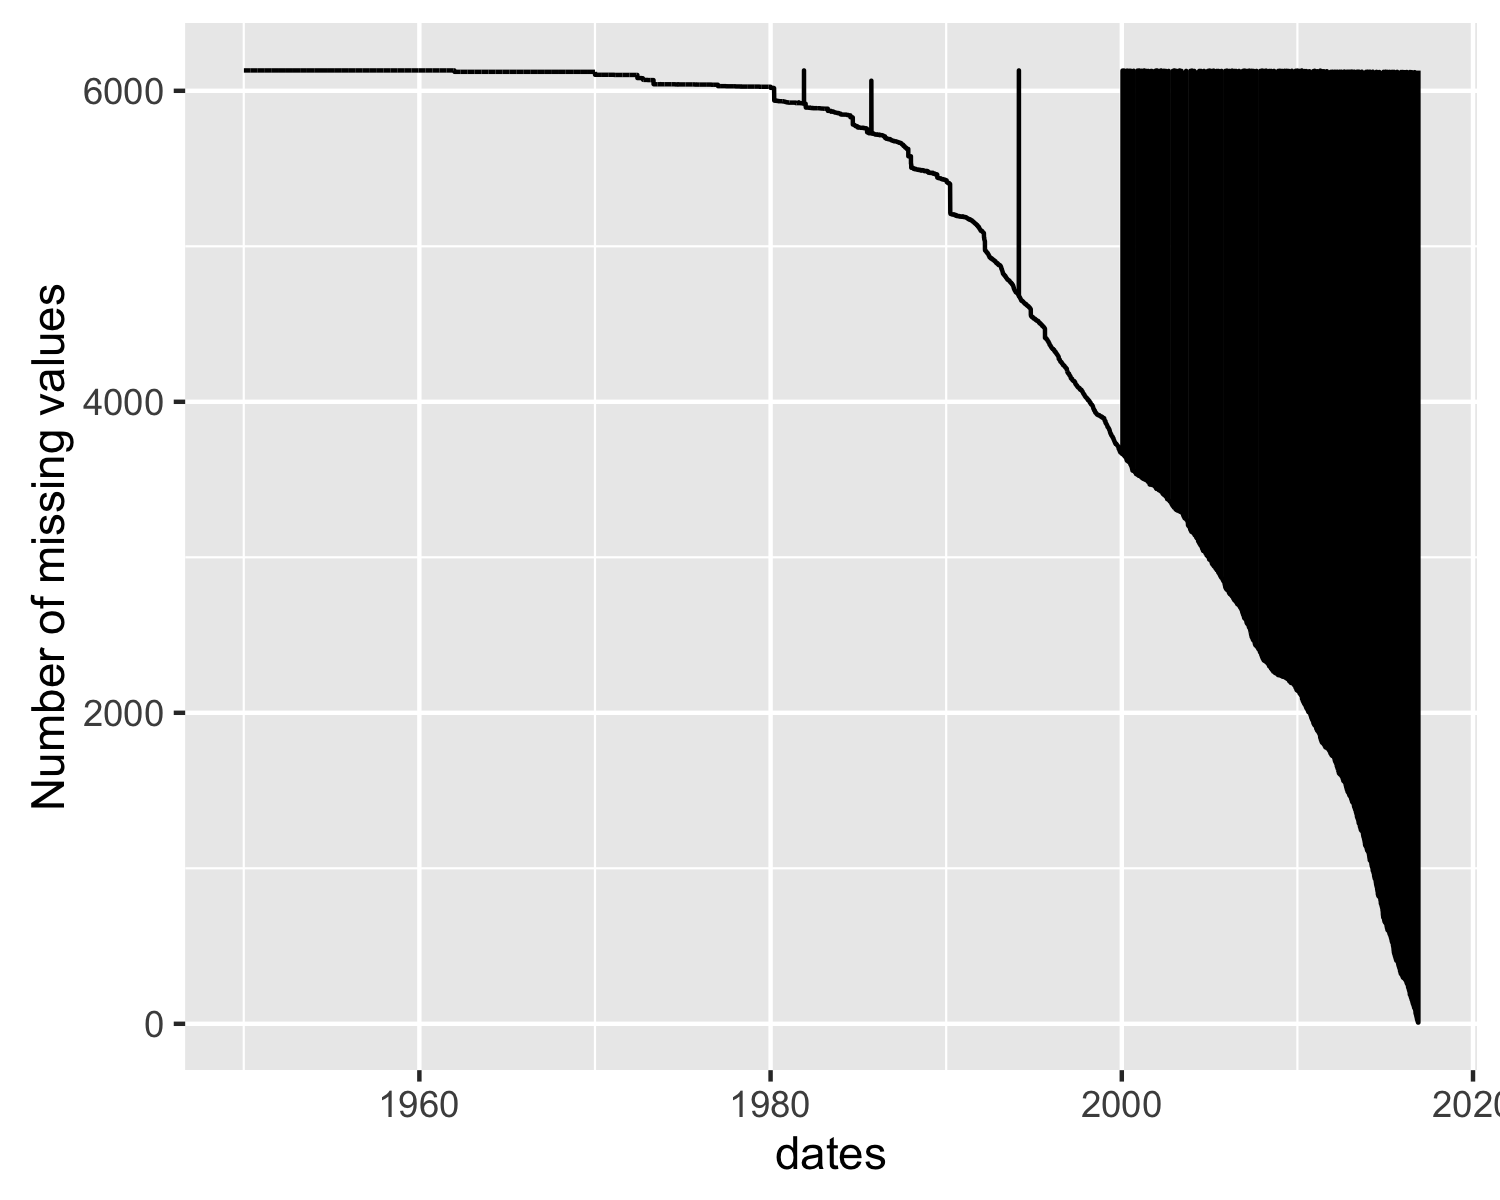
\includegraphics[width=0.45\textwidth]{fig0.png}}
  \caption{Number of missing values as a function of date.\label{fig:fig0}}
\end{figure}

\section{Statistical exploration of assets returns}

This section is trying to unveil some typical characteristics of financial market data. These are summarized in the literature as "stylized facts"~\cite{Rama}. Almost all return time series of stocks and indexes exhibit the same statistical properties. A risk model that does not capture the characteristics of the financial market data will not be useful for deriving risk measures. The main stylized facts are: 
\begin{itemize}
\item the absence of simple arbitrage
\item the power law decay of the tails of the return distribution
\item the volatility clustering
\end{itemize}
In the following sections we check whether these stylized facts are applicable to the daily log returns of Apple stock and S\$P500 index. Before proceeding further, log return for a particular day is given by $ret_t = log(p_t/p_{t-1})$ where $p_t$ denotes price on date $t$. Campbell et al.(1997)~\cite{Campbell} give reasons why returns are preferred instead of prices.

\subsection{Absence of simple arbitrage}

The absence of arbitrage implies that it is impossible to make profits in financial markets without dealing with a risky investment. In other words the market is efficient in the sense that it quickly tries to eliminate arbitrage opportunities. The price series up to now gives no information about the next asset price. The autocorrelation function of returns is assumed as a good measure of the market efficiency. We report the autocorrelation of returns for the Apple stock in figure \ref{fig:fig1}. It is seen in figure \ref{fig:fig1} how the autocorrelation function for the Apple returns series decays to zero after one lag. 


\begin{figure}[!tbp]
  \centering
  \begin{minipage}[t]{0.45\textwidth}
    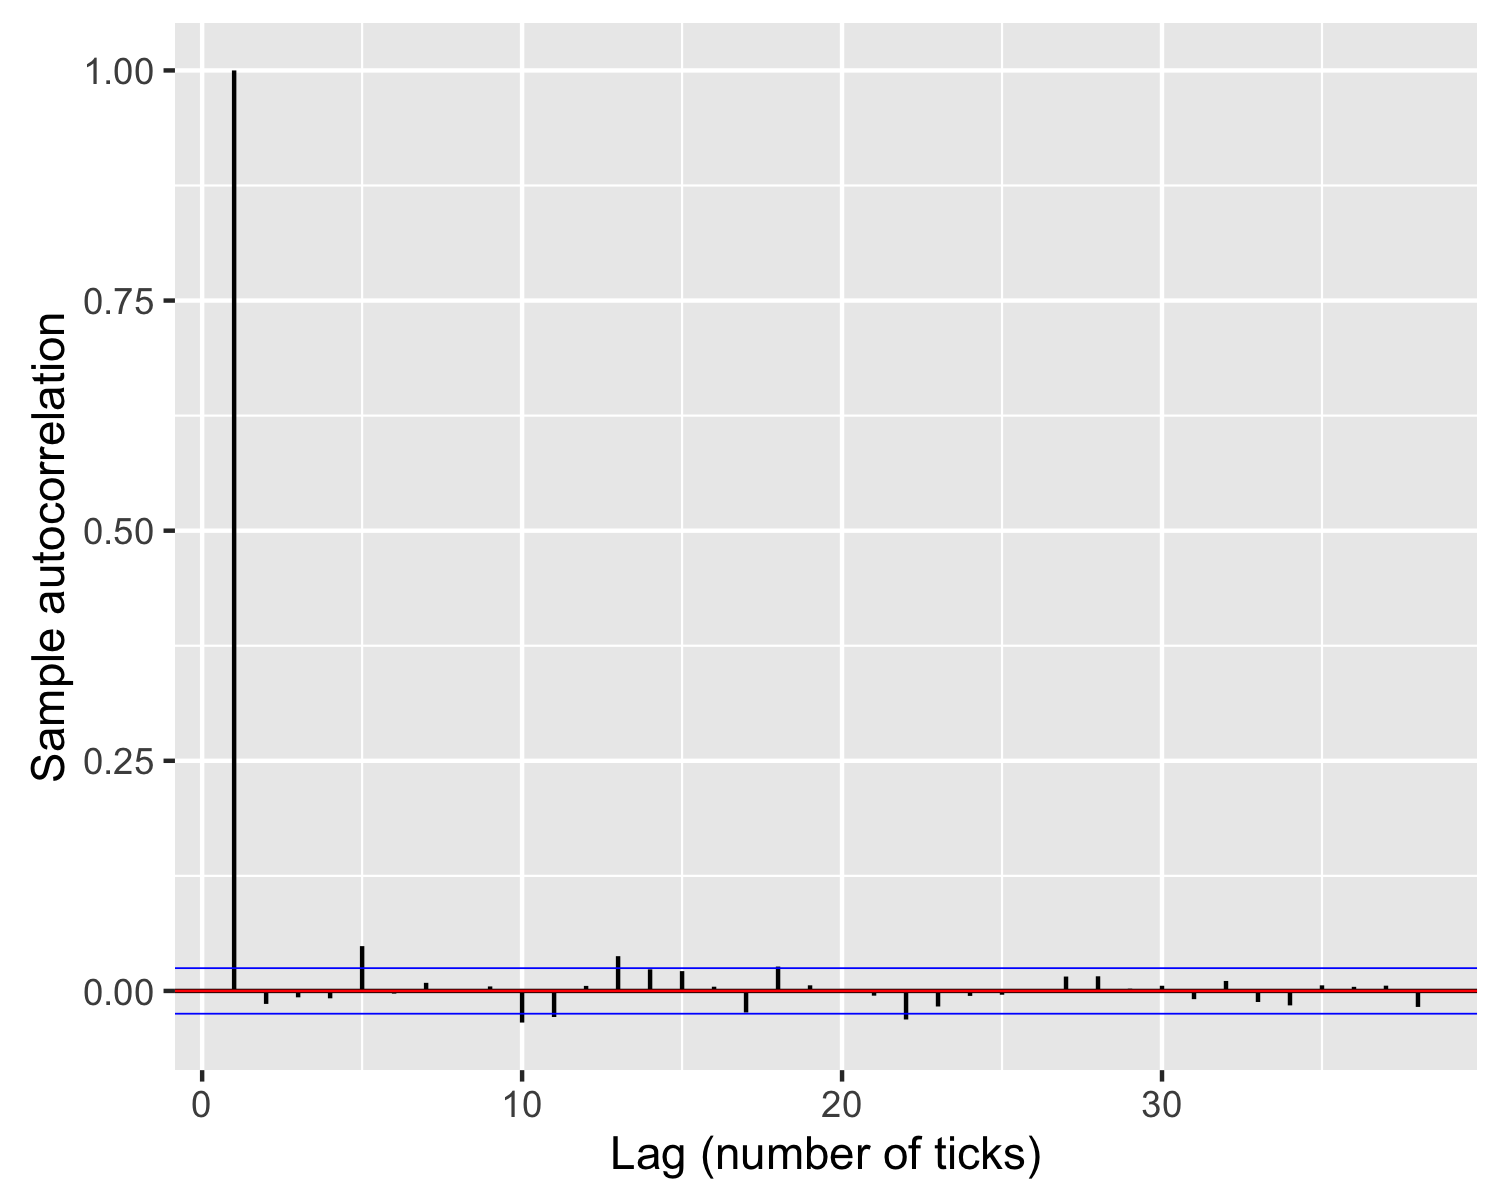
\includegraphics[width=\textwidth]{fig1.png}
    \caption{Autocorrelation function of tick by tick returns on Apple shares traded on the NYSE. Time scale: ticks.\label{fig:fig1}}
  \end{minipage}
  \hfill
  \begin{minipage}[t]{0.45\textwidth}
    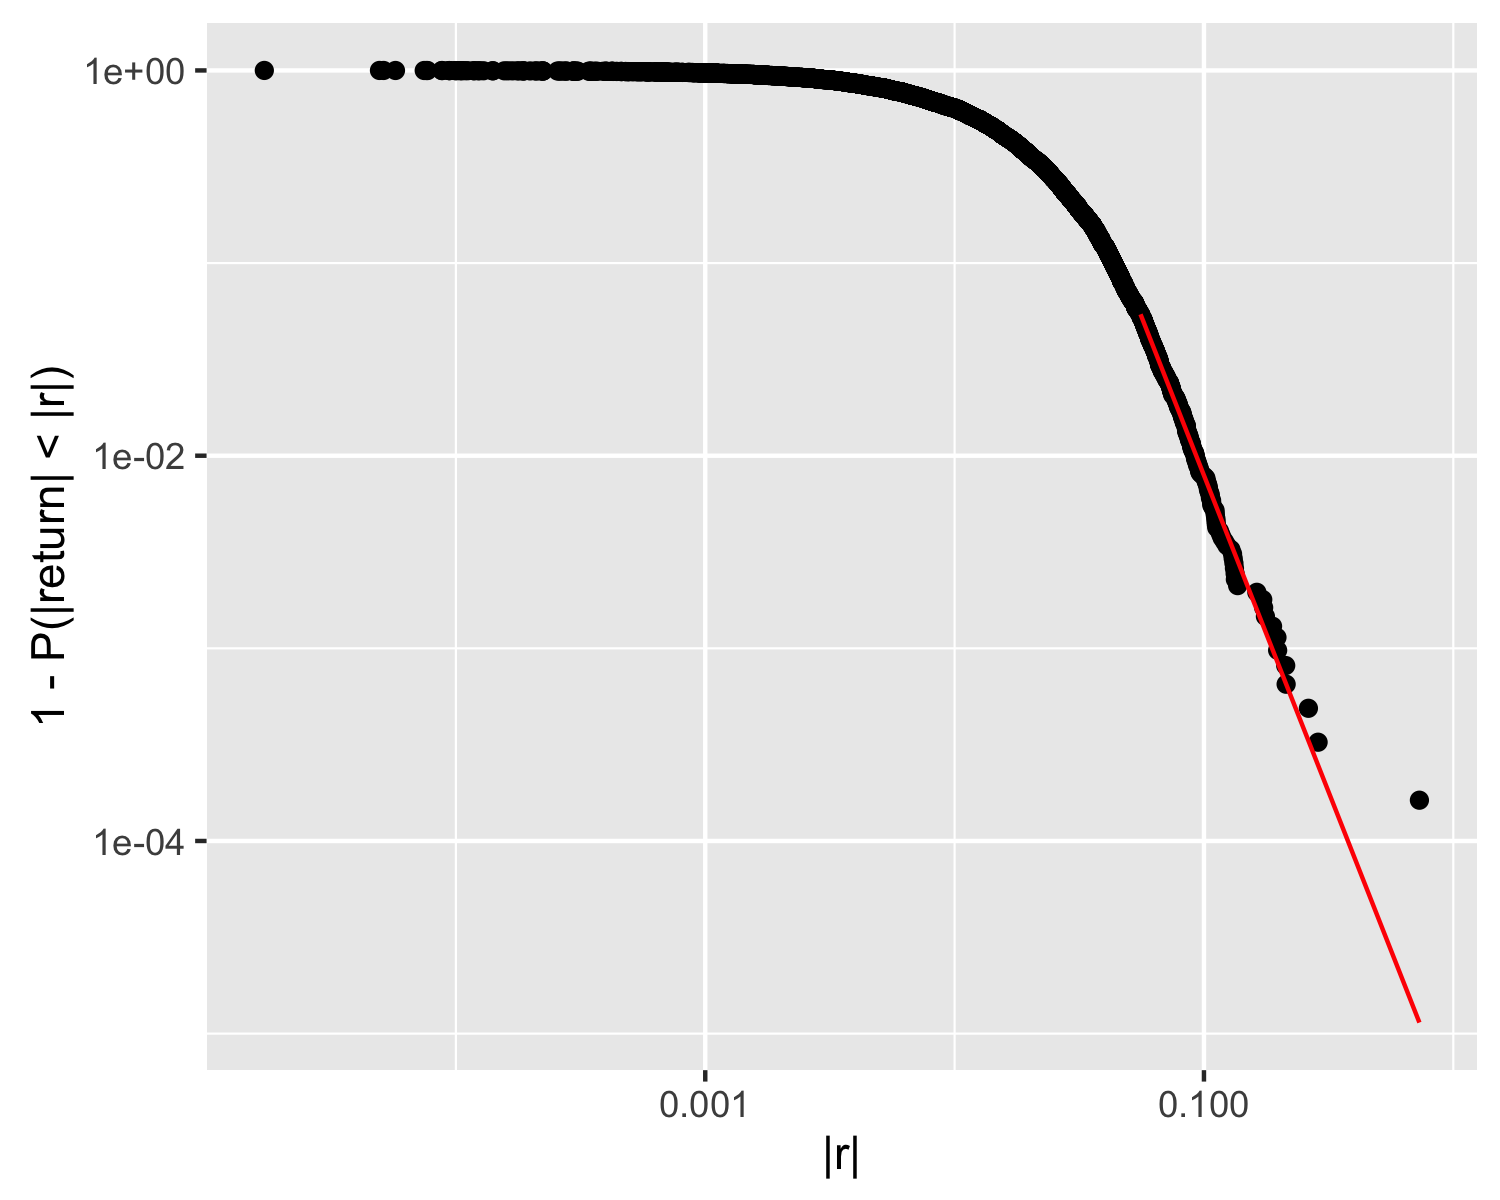
\includegraphics[width=\textwidth]{fig2.png}
    \caption{CDF of Apple returns with line of best fit.\label{fig:fig2}}
  \end{minipage}
\end{figure}


\subsection{Fat-Tailed distribution of returns}

The distribution of returns is not a Gaussian and prices do not follow a simple random walk. In details very large fluctuations are much more likely in stock market with respect to random walk and dramatic crashes are approximately observed every 5-10 years on average. These large events cannot be explained by gaussian returns. Therefore to characterize the probability of these events we introduce the complementary cumulative distribution function $F(x)$: 

\[ F(x) = 1 - Prob(X < x) \]
which describes the tail behavior of the distribution P(x) of returns. The complementary cumulative distribution function $F(x)$ of real returns is found to be approximately a power law $F(x) \sim\  x^{-a}$ with exponent in the range 2-5 ~\cite{Rama}, i.e. the tails of the probability density function (pdf) decay with an exponent $a + 1$. Since the decay is much slower than a gaussian this evidence is called Fat or Heavy Tails. Moreover the return pdf is characterized by large kurtosis, whereas a gaussian is characterized by kurtosis equals to three. In our case (Apple returns) $a = 4.28$ and $kurtosis = 6.52$. In figure \ref{fig:fig2} we report the complementary distribution function $F(x)$ of Apple returns with the best fit.

\begin{figure}[!tbp]
  \centering
  \begin{minipage}[t]{0.45\textwidth}
    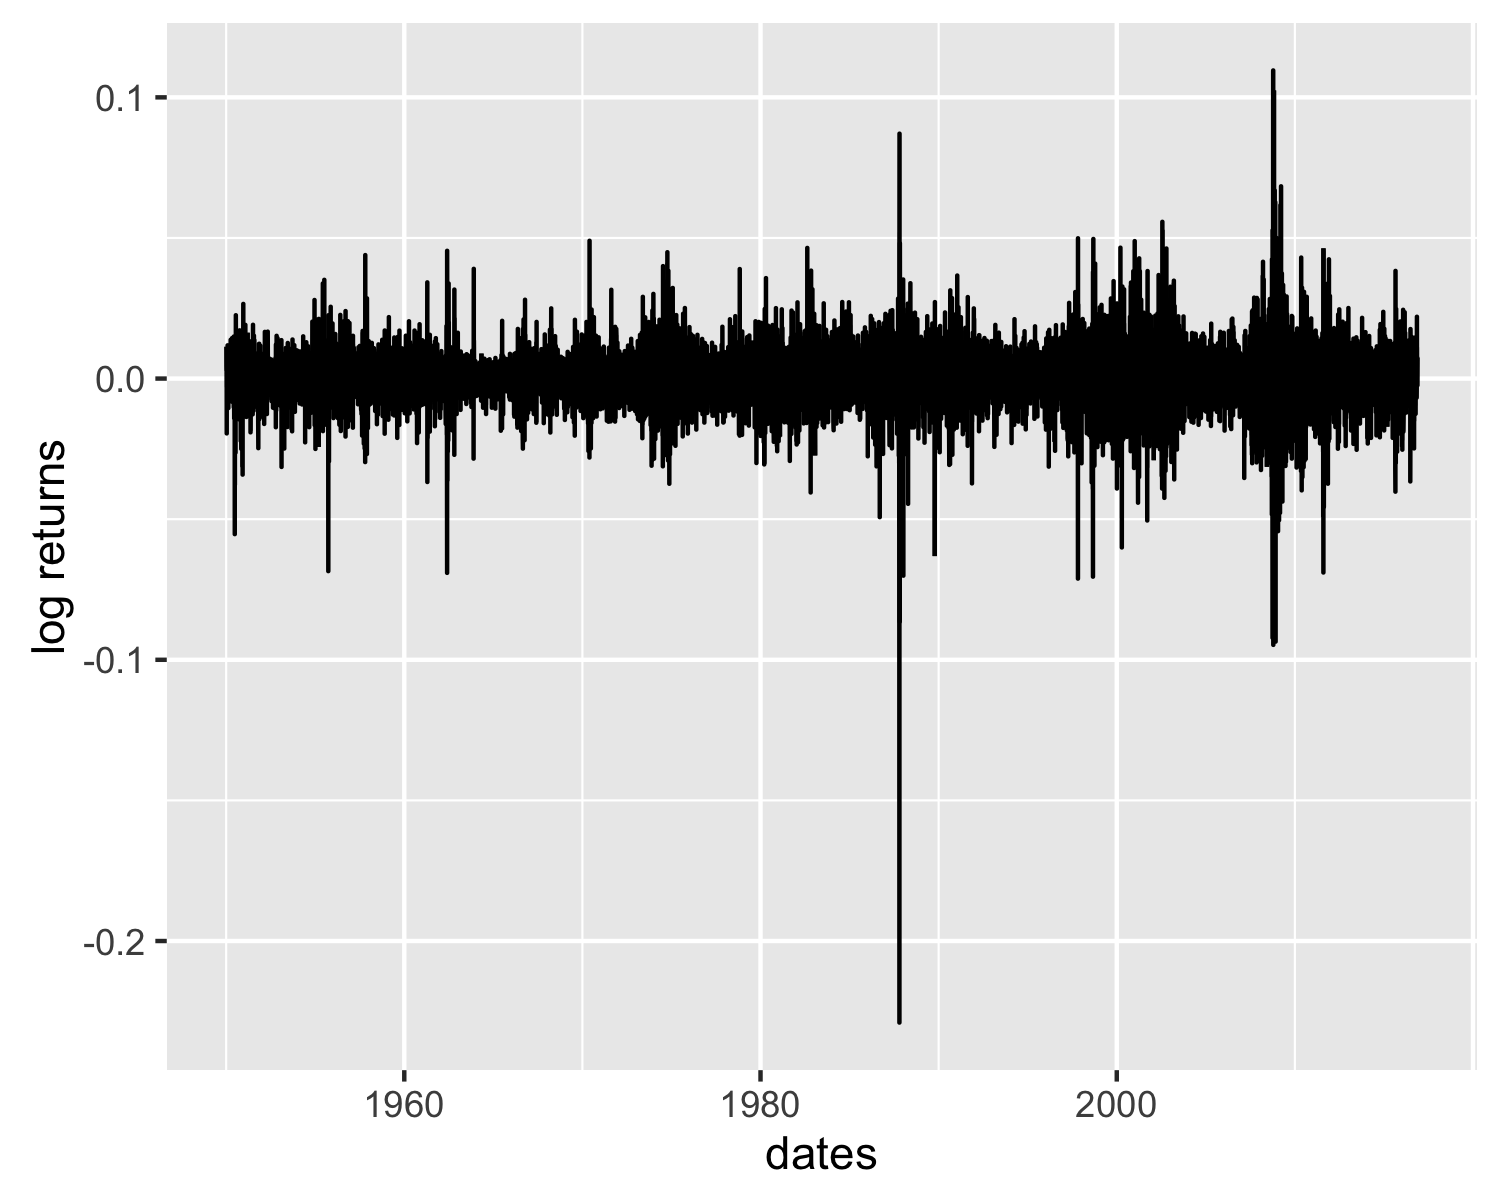
\includegraphics[width=\textwidth]{fig3.png}
    \caption{Log returns of S\&P500 for period 1950-2016.\label{fig:fig3}}
  \end{minipage}
  \hfill
  \begin{minipage}[t]{0.45\textwidth}
    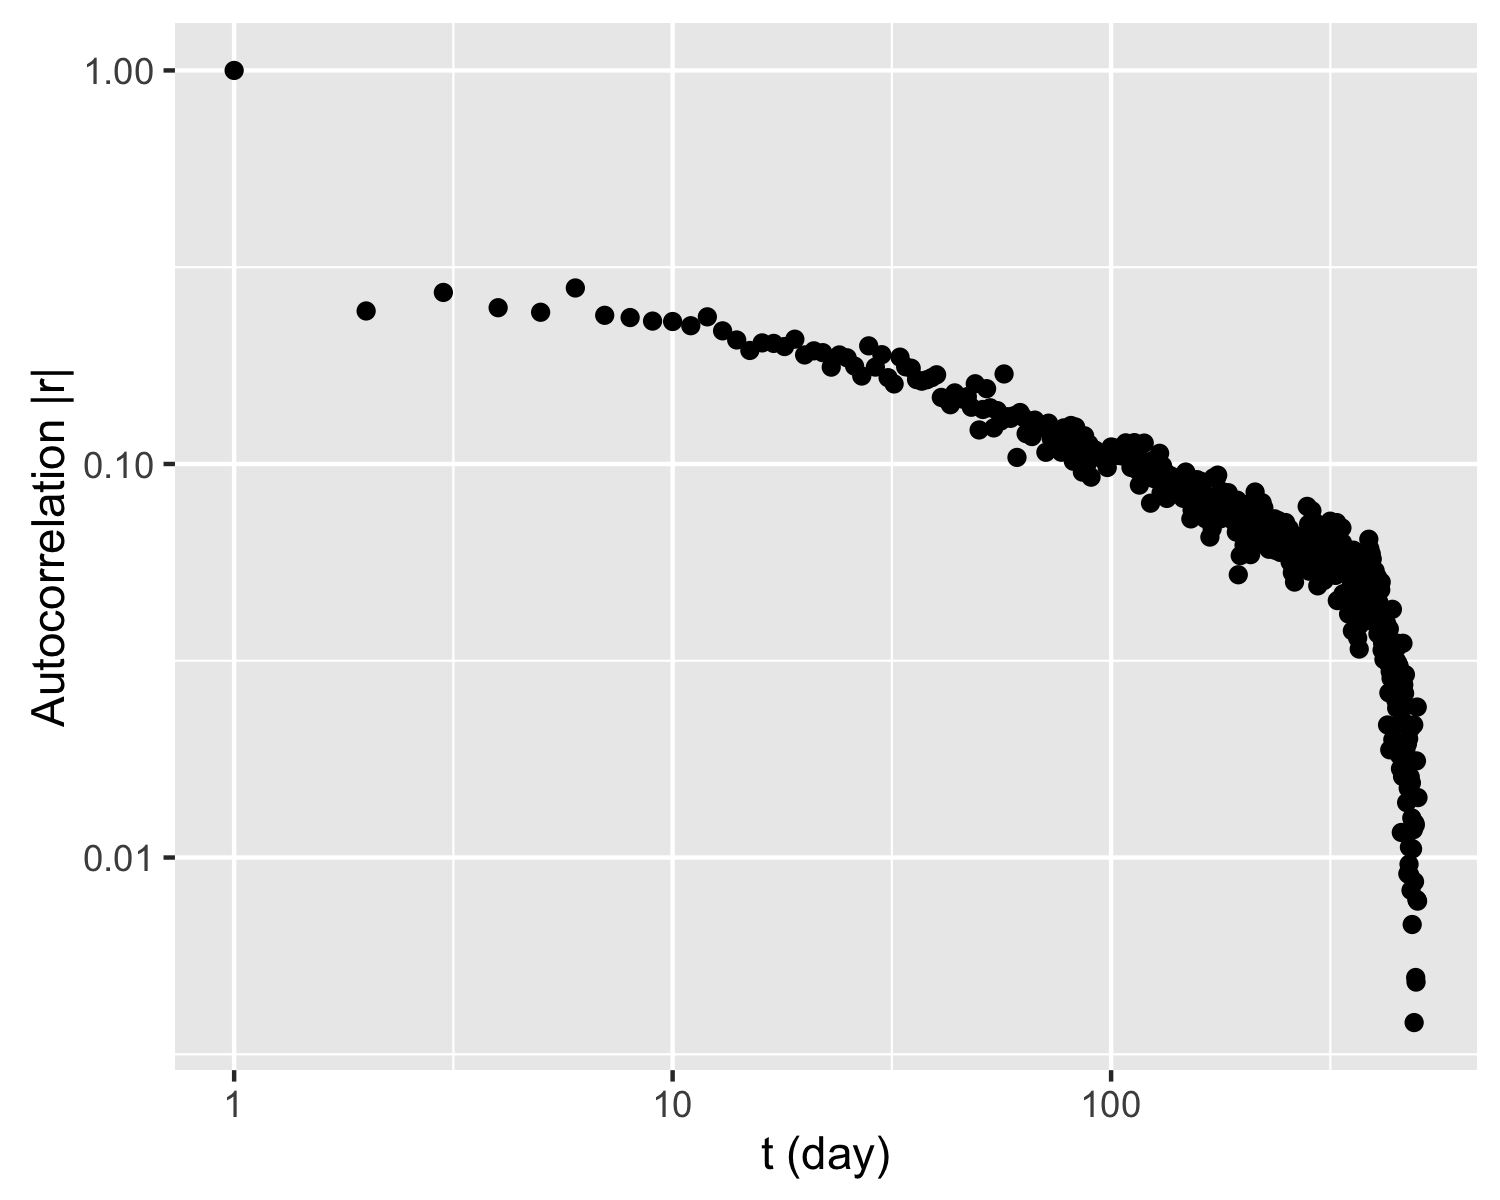
\includegraphics[width=\textwidth]{fig4.png}
    \caption{Autocorrelation function of volatility measured as the absolute value of returns for returns of S\&P500 for period 1950-2016.\label{fig:fig4}}
  \end{minipage}
\end{figure}

\subsection{Volatility Clustering}

We report the return time series of the S\&P500 index for period 1950-2016. It is clear from figure \ref{fig:fig3} that periods of large fluctuations are followed by large fluctuations regardless of the sign and the same behavior happens for small ones. As a consequence the autocorrelation function of absolute returns is non zero. This is presented in figure \ref{fig:fig4}. The very slow decay means that volatility is correlated on very long time scales from minutes to several months/years. The autocorrelation function of absolute returns decays slowly as a function of the time lag, roughly as a power law with an exponent $\beta \in [0.2, 0.4]$. The volatility clustering was observed the first time by Mandelbrot~\cite{Mandelbrot}.

\subsection{Other Stylized Facts}

We can present other effects that are widespread in financial markets such as:

\begin{itemize}
\item Gain loss asymmetry: one observes large drawdowns in stock prices and stock index values but not equally large upward movements. This is linked to the asymmetry of the return pdf. To prove this we calculate the skewness and the kurtosis of daily log returns of S\&P 500 for the period 1950-2016. $Kurtosis = 27.09$ indicating fat tails, and $skewness = -1.01$ indicating the lack of symmetry. Concretely our skewness is negative, i.e. we have frequent small gains and a few extreme losses.   
\item Aggregational Gaussianity: as ones increases the time scale over which returns are calculated, their distribution looks more and more like a normal distribution. Table \ref{table:tbl1} shows how kurtosis and the value of Jarque-Bera normality test decreases as time scale increases. Jarque-Bera normality test determines if assets historical returns' probability distribution skewness and kurtosis match a standard normal probability distribution.

\begin{table}[]
\centering
\caption{Summary statistics for S\&P500 returns from 1950 to 2016}
\label{table:tbl1}
\begin{tabular}{cccccccc}
\hline
\textbf{Time Scale} & \textbf{Mean} & \textbf{Median} & \textbf{Std} & \textbf{Skewness} & \textbf{Kurtosis} & \textbf{JB} & \textbf{JB p-value} \\ \hline
Daily               & 0.00029             & 0.00046               & 0.00970            & -1.01057                 & 27.09344               & 518160         & \textless 2.2e-16               \\
Weekly              & 0.00139             & 0.00307               & 0.02126            & -0.63072                 & 5.524142               & 4691.2         & \textless 2.2e-16                 \\
Monthly             & 0.00608             & 0.00906               & 0.04155            & -0.65472                 & 2.452925               & 264.16         & \textless 2.2e-16                 \\
Quarterly           & 0.01821             & 0.02723               & 0.07728            & -0.96021                 & 2.012611               & 91.008         & \textless 2.2e-16                 \\
Annually            & 0.07287             & 0.10787               & 0.16253            & -0.93114                 & 1.139258               & 15.832         & 0.013                 \\ \hline
\end{tabular}
\end{table}



\end{itemize}

\section{Analysis based on Covariance Matrix}
\par There exists many long-term quantitative strategies such that \textbf{Modern portfolio theory or mean-variance analysis}~\cite{Markowitz} introduced by Harry Markowitz and \textbf{asset allocation} ~\cite{Asset}. All these methods of building your portfolio are proved to be wrong at many cases. Moreover the conjecture that the risk premium is non negative and increasing is at most times not true. This conjecture justifies the mean-variance portfolio optimization. So in a world with zero risk premium the optimal portfolio is not the mean-variance portfolio but the minimum-variance portfolio. In this optimization method security weights are independent of the expected security returns ~\cite{Min-variance}. In our analysis we try both mean-variance and minimum-variance portfolio optimization. \newline
The first step in every kind of analysis is to compute a rolling window covariance matrix. We choose the size of the window to be 2000 ($\approx 2 * number\ of\ stocks$). More concretely we calculate the covariance matrices for all the dates that Stock Exchange was open between 18.12.2007 - 21.11.2016 using the 2000 previous dates. So we end up with 2249 covariance matrices. The size of every matrix is 1018 x 1018, as we have 1018 ticker symbols in our dataset. We use the R package WGNA ~\cite{WGCNA}, a package that calculates correlation matrix in a very efficient way. After that step we can optimize out portfolio. But the problem is that the calculated covariance matrix is not \textbf{positive definite} to ensure the optimization problem is convex. So we could not solve the optimization problem with this covariance matrix. By using the R package \href{https://cran.r-project.org/web/packages/Matrix/Matrix.pdf}{Matrix} and its function nearPD, we are able to calculate the nearest positive definite matrix to our initial covariance matrix and thus to overcome our problem. \newline
As mentioned in class nobody should be using the sample covariance matrix for the purpose of portfolio optimization. It contains estimation error of the kind most likely to perturb a mean-variance optimizer. There is a method called shrinkage ~\cite{LW} that transforms the sample covariance matrix into a matrix that can be used to optimize our portfolio. One advantage of this method is that the matrix is always positive definite. Both in minimum-variance portfolio and in mean-variance portfolio we compare the expected return and the volatility when using the sample covariance matrix and the matrix after shrinkage.

\subsection{Minimum variance Portfolio}
As already mentioned, the minimum variance portfolio is the optimal portfolio if we assume that the risk premium is equal to zero. The classic Markowitz mean-variance optimal portfolio is the solution to:

$$\min\limits_{w} w^T\Omega w - \frac{1}{\gamma}\mu^T w$$

$$Subject\ to: \sum_{i} w_i$$


where $w \in R^n$ are vectors of portfolio weights, $\mu^T w$ is sample mean portfolio return, and $w^T\Omega w$ is sample covariance of the portfolio returns. The constraint (summation equals to one) ensure that the investor invests all his money meaning full investment. Also we don't allow short selling, which adds the following non-negative optimization constraint:

$$\forall i : w_i \geq 0$$

Also by assuming that the risk premium is zero, is equivalent that the aversion to risk is infinite, thus $\gamma \to \infty$. With all those assumptions, the above optimization problem reduces to the following problem:

$$\min\limits_{w} w^T\Omega w$$

$$Subject\ to: \sum_{i} w_i$$

We construct the portfolio only with stocks. In order to minimize the idiosyncratic risk we set an upper bound $\epsilon$ to every weight $w_i$, and to avoid having only a few stocks in our portfolio.\newline
R package \href{https://cran.r-project.org/web/packages/quadprog/quadprog.pdf}{quadprog} and its function solve.QP is used for portfolio optimization. So we get weights for every date between 18.12.2007 - 21.11.2016. At an average our model chooses approximately 80 ticker symbols in order to minimize the variance, therefore the risk. In figure \ref{fig:fig_min_variance_ins_r} we report the daily in-sample expected return, and in figure \ref{fig:fig_min_variance_ins_std} the corresponding standard deviation. We perform backtesting to evaluate the performance of the optimized portfolio. To do this we choose a second part of stock returns from our dataset and we call it out of sample evaluation sample. By separating the estimation sample and the evaluation sample we give a realistic assessment of the performance of the portfolio. It is crucial that there is no overlap between the estimation sample and the evaluation sample. Otherwise there is a look ahead bias. This means that we are optimizing the portfolio using more information than we actually have at the time of the investment decision. Such a look ahead bias leads to a too optimistic view on how good the optimized portfolio performs in real life. We choose a window of 200 for our evaluation sample. For example suppose we are in date 18.12.2007, we evaluate our portfolio in the returns that happened between the dates 19.12.2007 - 03.10.2008 (200 days). The results for out-of-sample expected returns and standard deviations are presented in figures \ref{fig:fig_min_variance_ous_r}, \ref{fig:fig_min_variance_ous_std} Also the out-of-sample cumulative expected return is presented in figure \ref{fig:fig_min_variance_cum}.


\begin{figure}[!tbp]
  \centering
  \begin{minipage}[t]{0.45\textwidth}
    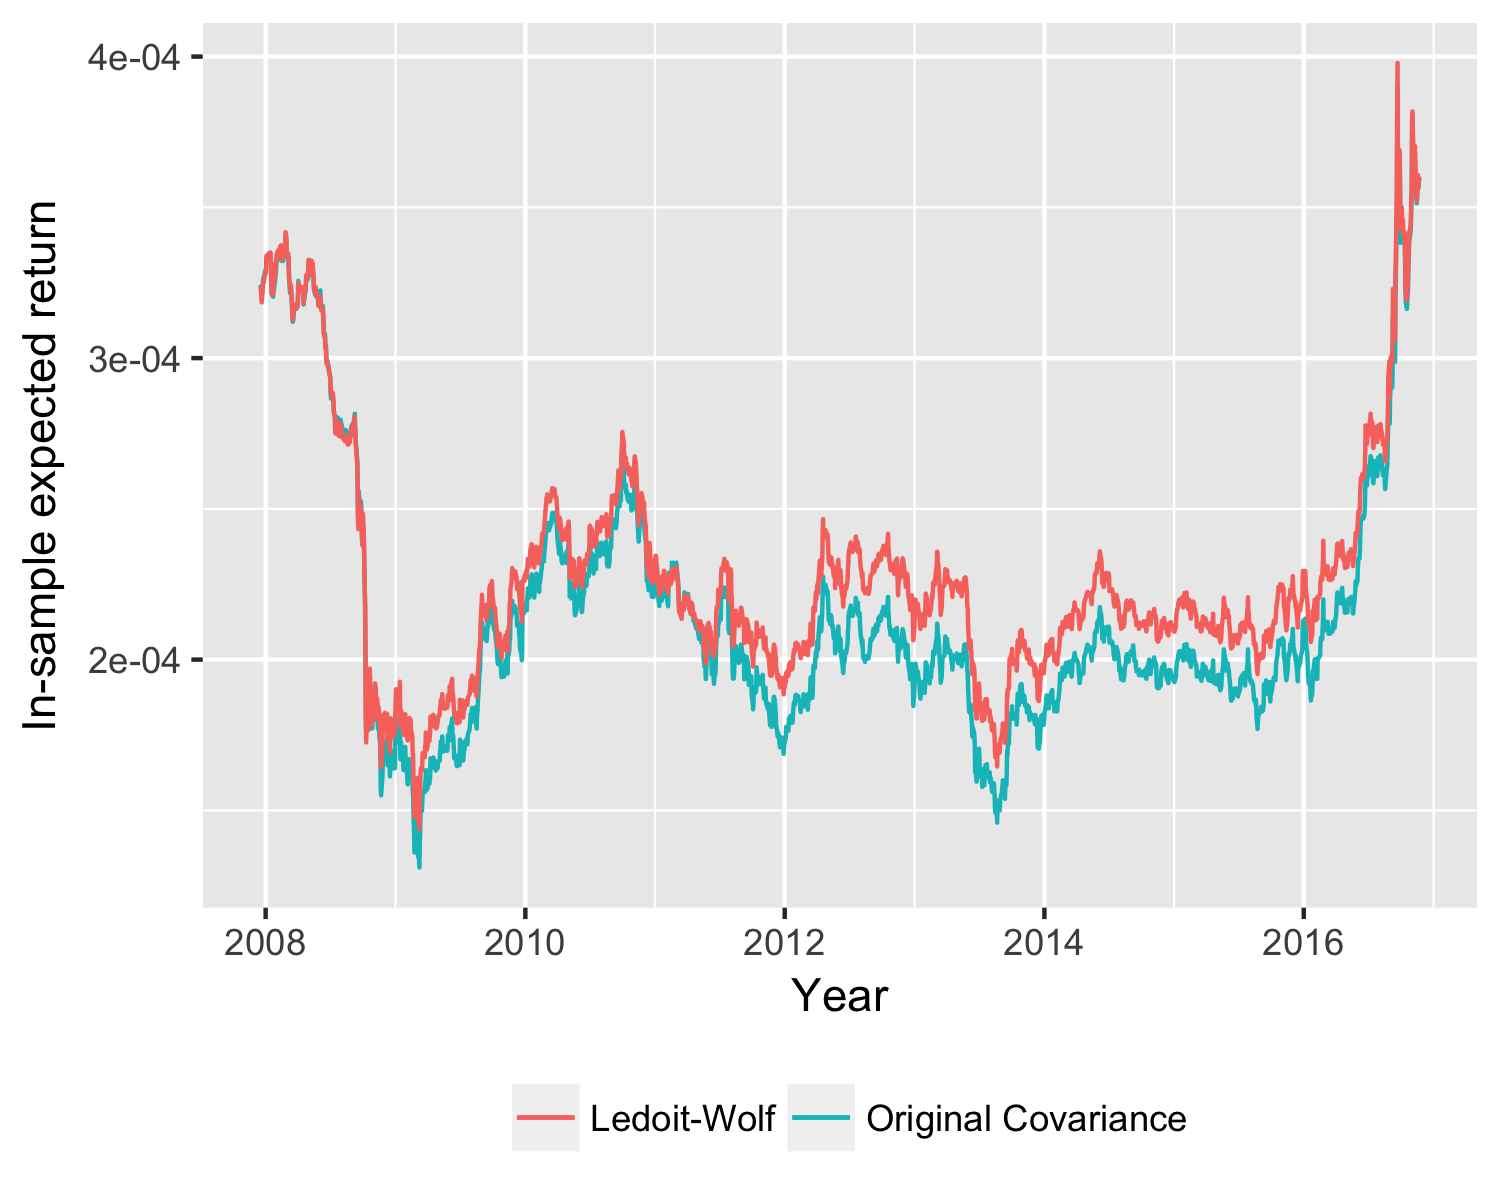
\includegraphics[width=\textwidth]{fig_min_variance_ins_r.png}
    \caption{In sample expected returns (minimum-variance portfolio).\label{fig:fig_min_variance_ins_r}}
  \end{minipage}
  \hfill
  \begin{minipage}[t]{0.45\textwidth}
    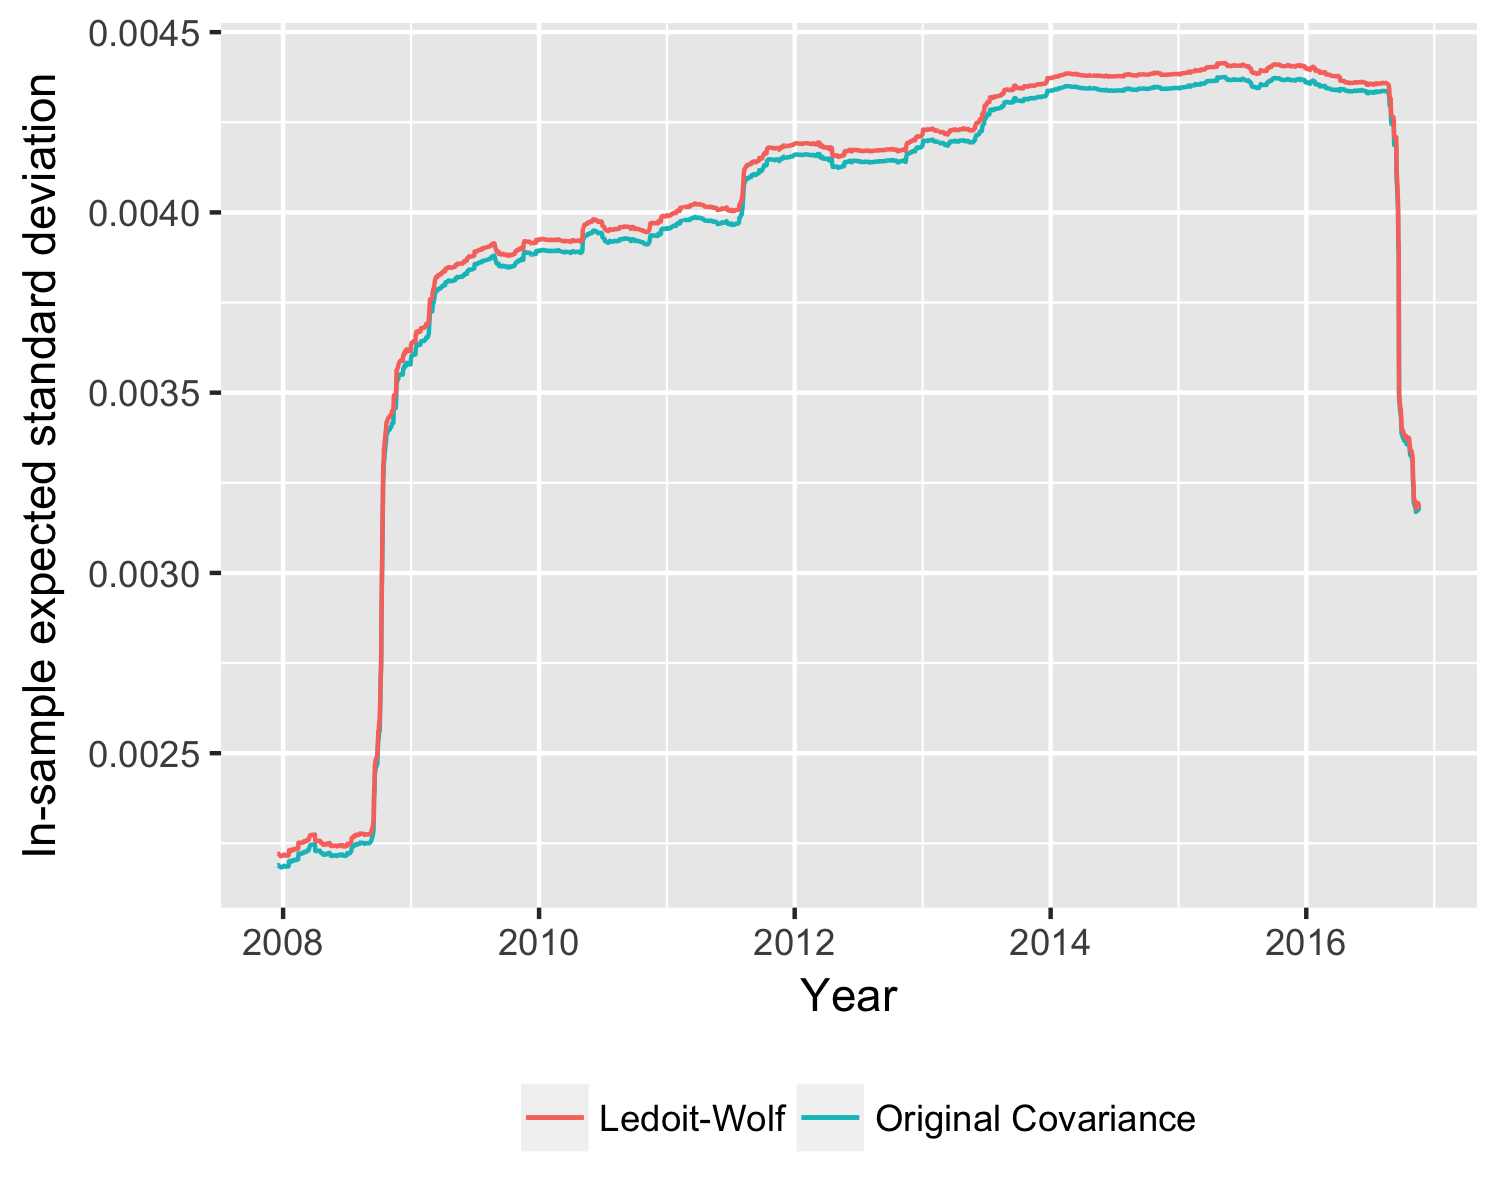
\includegraphics[width=\textwidth]{fig_min_variance_ins_std.png}
    \caption{In sample expected standard deviations (minimum-variance portfolio).\label{fig:fig_min_variance_ins_std}}
  \end{minipage}
\end{figure}


\begin{figure}[!tbp]
  \centering
  \begin{minipage}[t]{0.45\textwidth}
    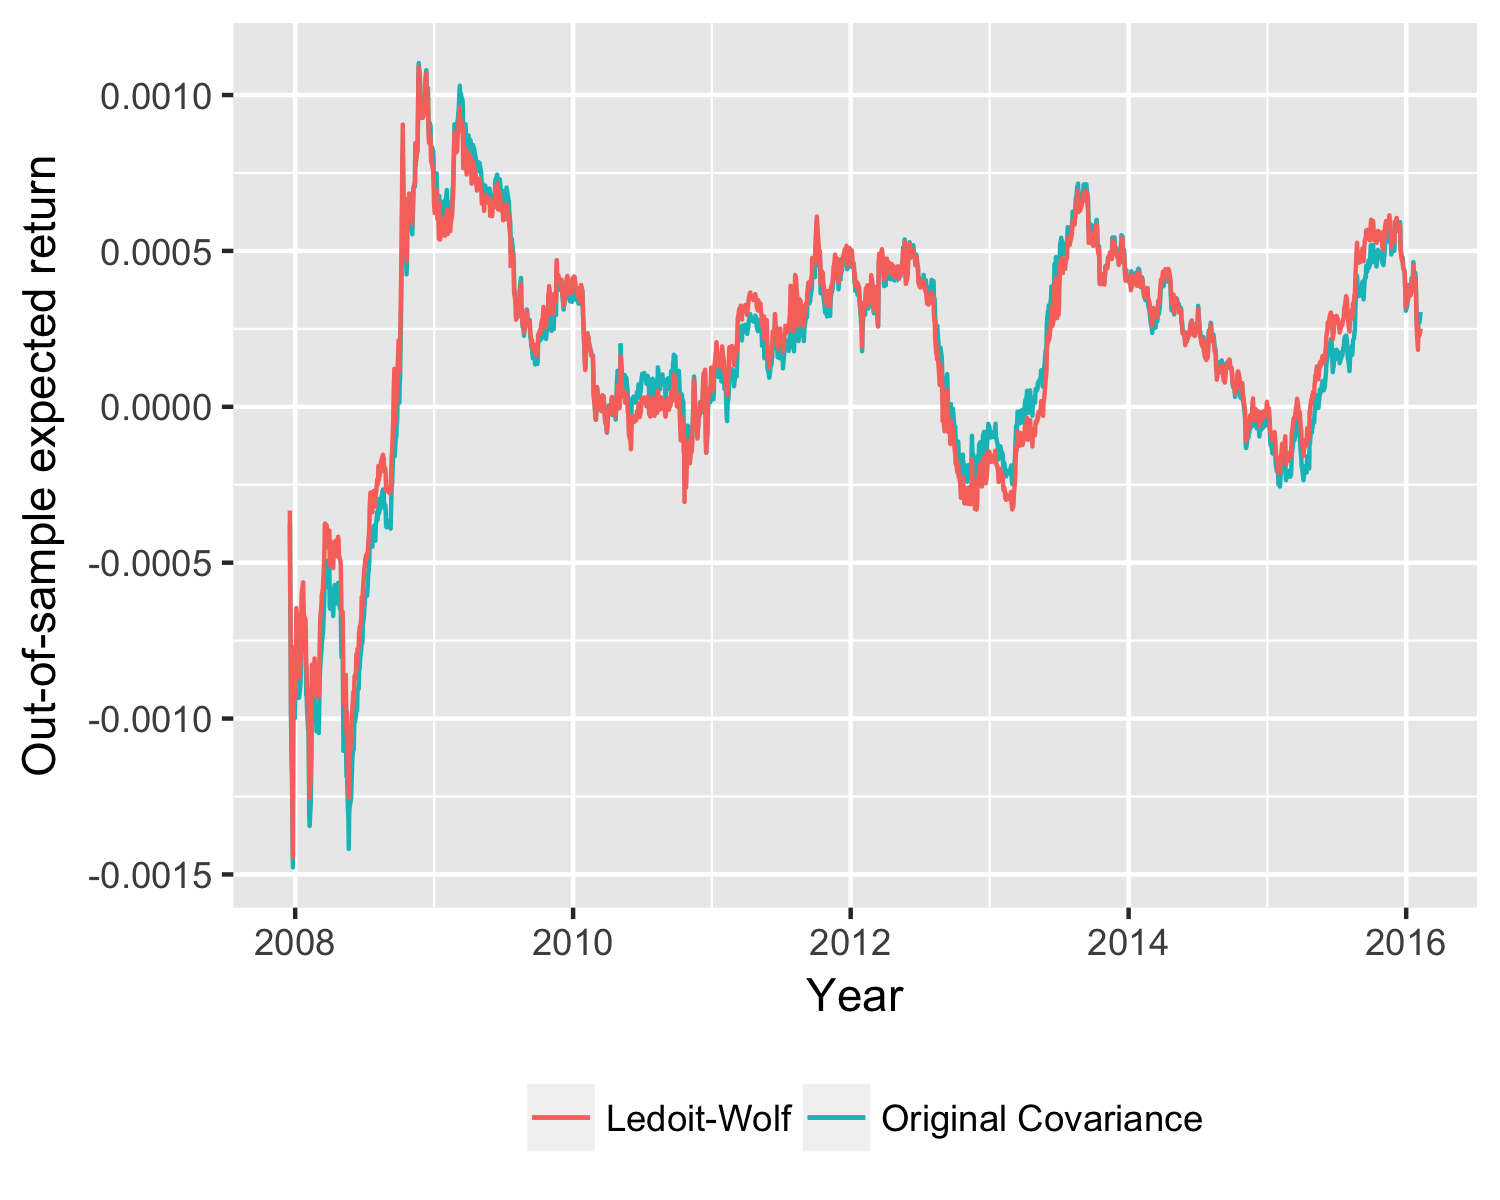
\includegraphics[width=\textwidth]{fig_min_variance_ous_r.png}
    \caption{Out of sample expected returns (minimum-variance portfolio).\label{fig:fig_min_variance_ous_r}}
  \end{minipage}
  \hfill
  \begin{minipage}[t]{0.45\textwidth}
    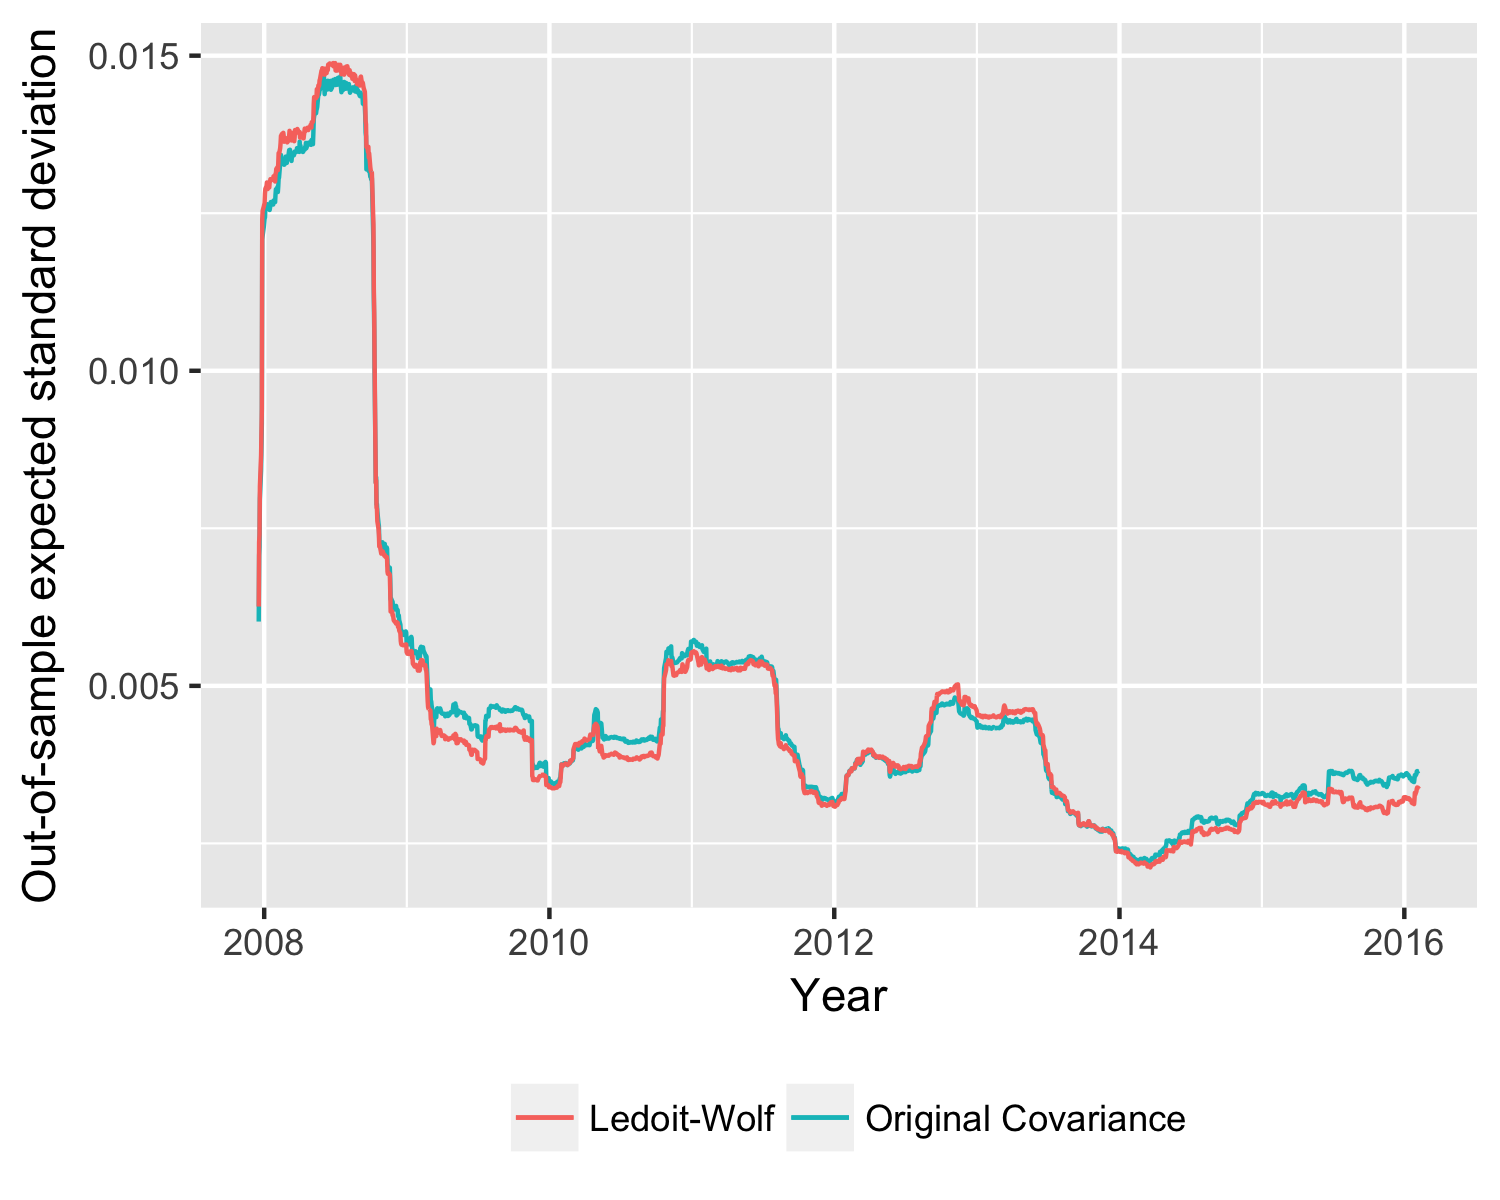
\includegraphics[width=\textwidth]{fig_min_variance_ous_std.png}
    \caption{Out of sample expected standard deviations (minimum-variance portfolio).\label{fig:fig_min_variance_ous_std}}
  \end{minipage}
\end{figure}

\begin{figure}
  \centering
    \centering{%
      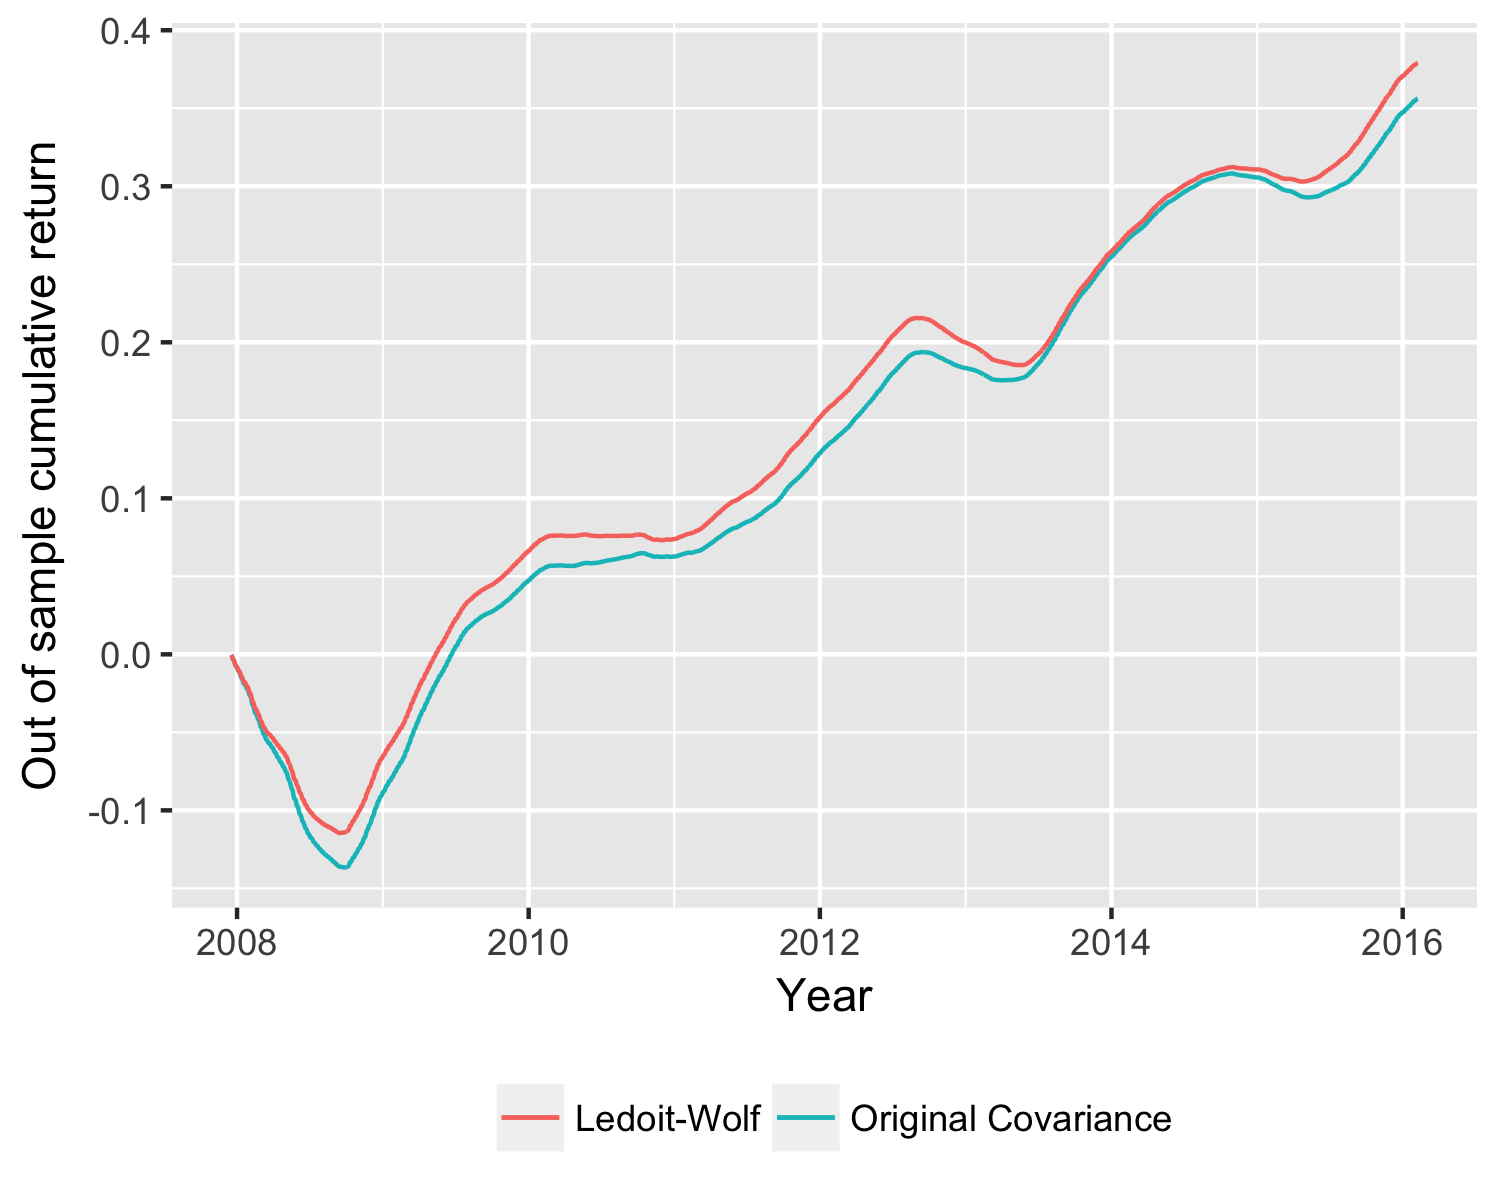
\includegraphics[width=0.45\textwidth]{fig_min_variance_cum.png}}
  \caption{Out of sample cumulative expected return (minimum-variance portfolio).\label{fig:fig_min_variance_cum}}
\end{figure}

\subsection{Mean variance Portfolio}
In this optimization problem, not only do we give as input to the function solve.QP the in-sample covariance matrix but also the in-sample expected returns of the ticker symbols, along with the constraints that we used when constructing the min-variance portfolio (no short sales, sum of weights equal to one, and upper bounded weights to avoid idiosyncratic risk). As in the previous portfolio optimization we calculate weights for both matrices and compare the results. In figure \ref{fig:fig_mean_variance_ins_r} we report the daily in-sample expected return, and in figure \ref{fig:fig_mean_variance_ins_std} the corresponding standard deviation. As usual we perform backtesting to evaluate the portfolio performance. The results for out-of-sample expected returns and standard deviations are presented in figures \ref{fig:fig_mean_variance_ous_r}, \ref{fig:fig_mean_variance_ous_std}. Also the out-of-sample cumulative expected return is presented in figure \ref{fig:fig_mean_variance_cum}.

\begin{figure}[!tbp]
  \centering
  \begin{minipage}[t]{0.45\textwidth}
    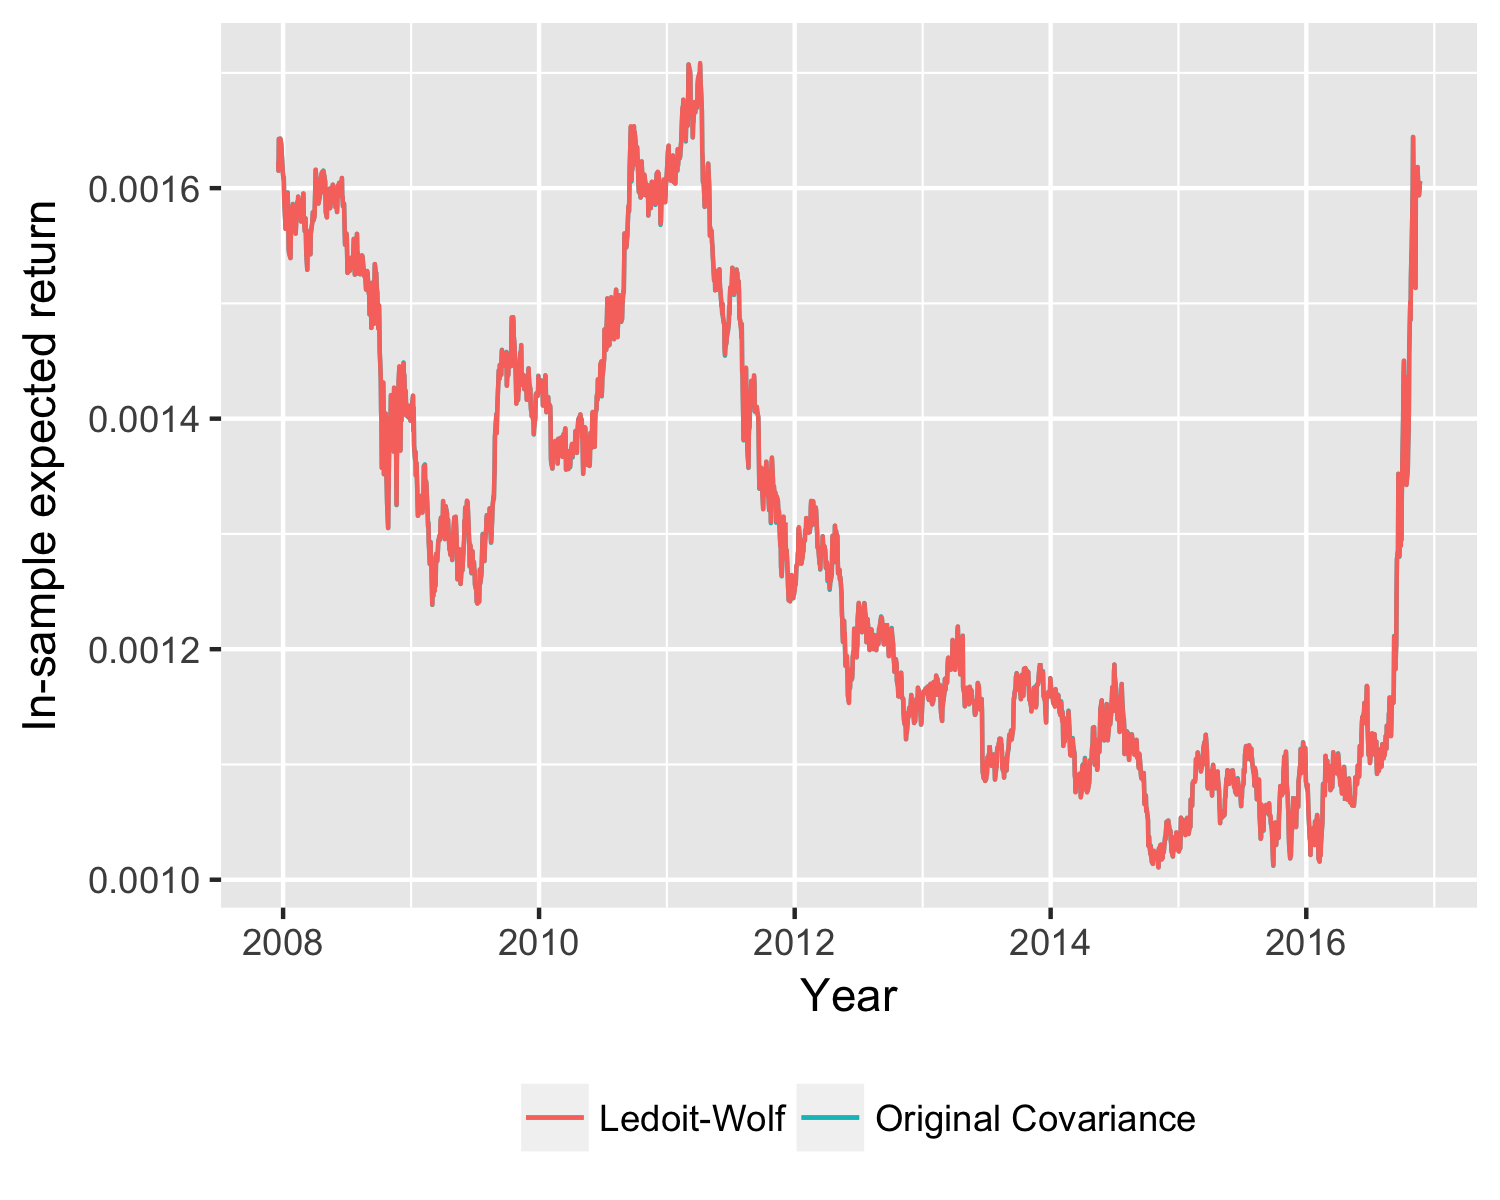
\includegraphics[width=\textwidth]{fig_mean_variance_ins_r.png}
    \caption{In sample expected returns (mean-variance portfolio).\label{fig:fig_mean_variance_ins_r}}
  \end{minipage}
  \hfill
  \begin{minipage}[t]{0.45\textwidth}
    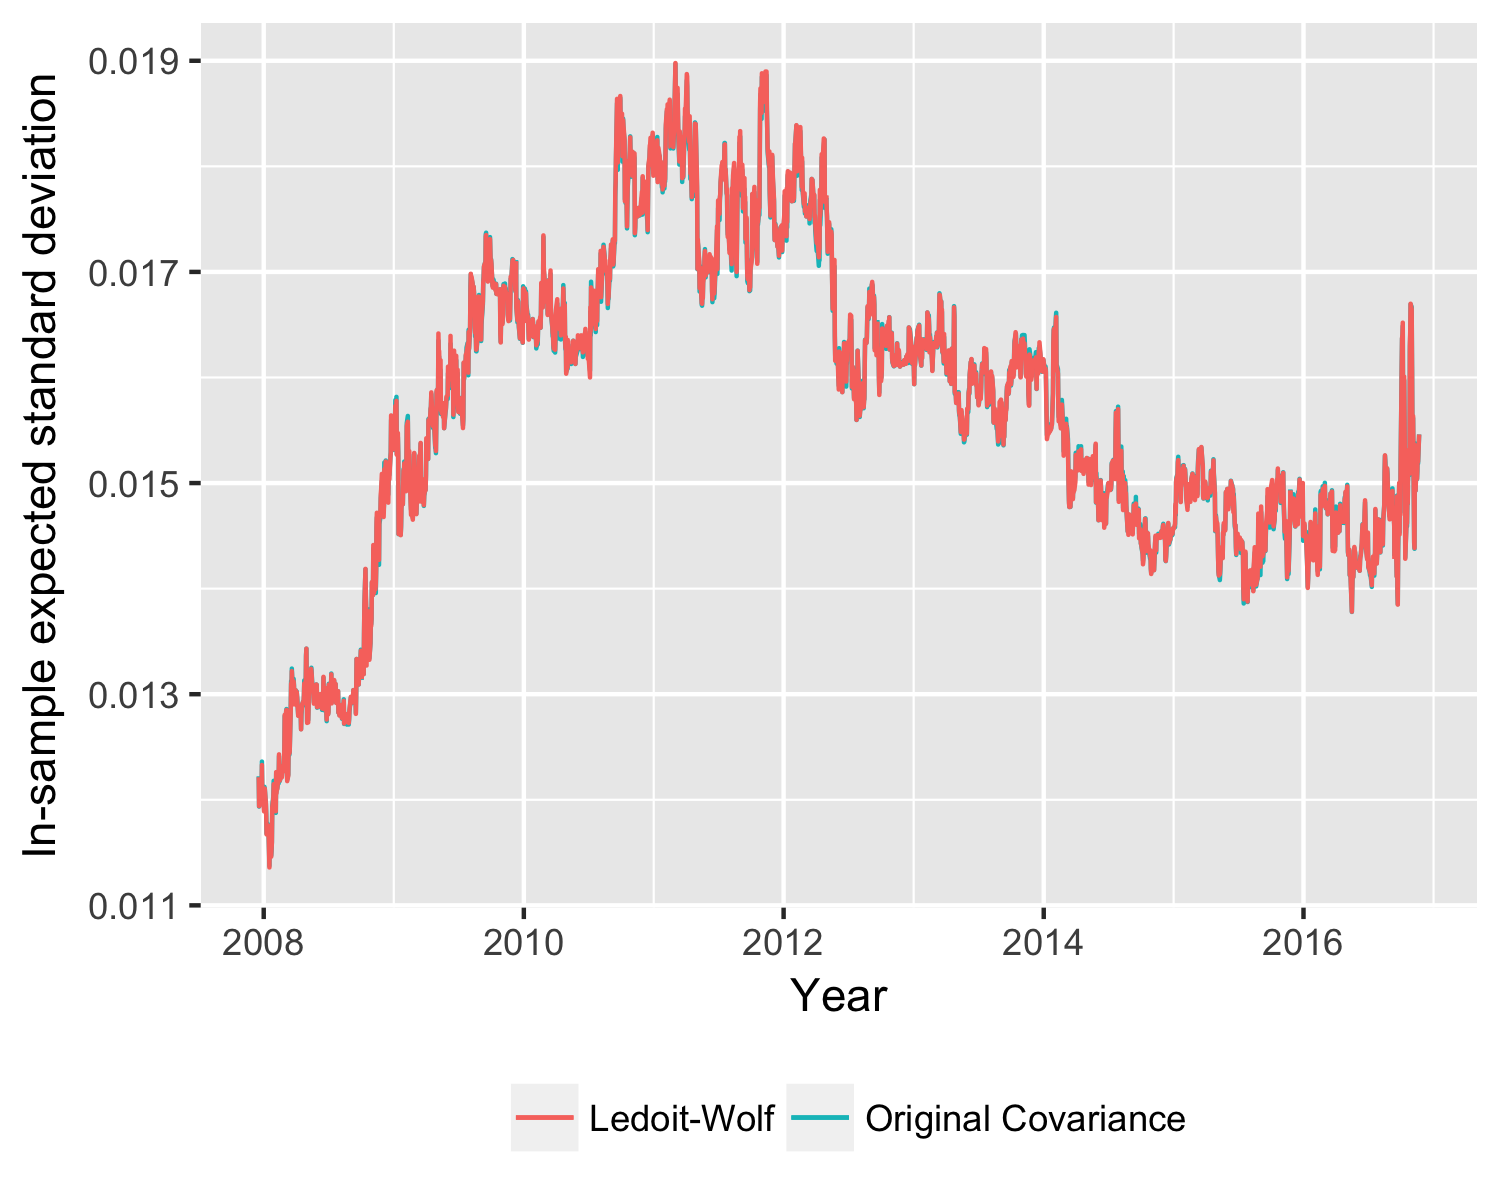
\includegraphics[width=\textwidth]{fig_mean_variance_ins_std.png}
    \caption{In sample expected standard deviations (mean-variance portfolio).\label{fig:fig_mean_variance_ins_std}}
  \end{minipage}
\end{figure}


\begin{figure}[!tbp]
  \centering
  \begin{minipage}[t]{0.45\textwidth}
    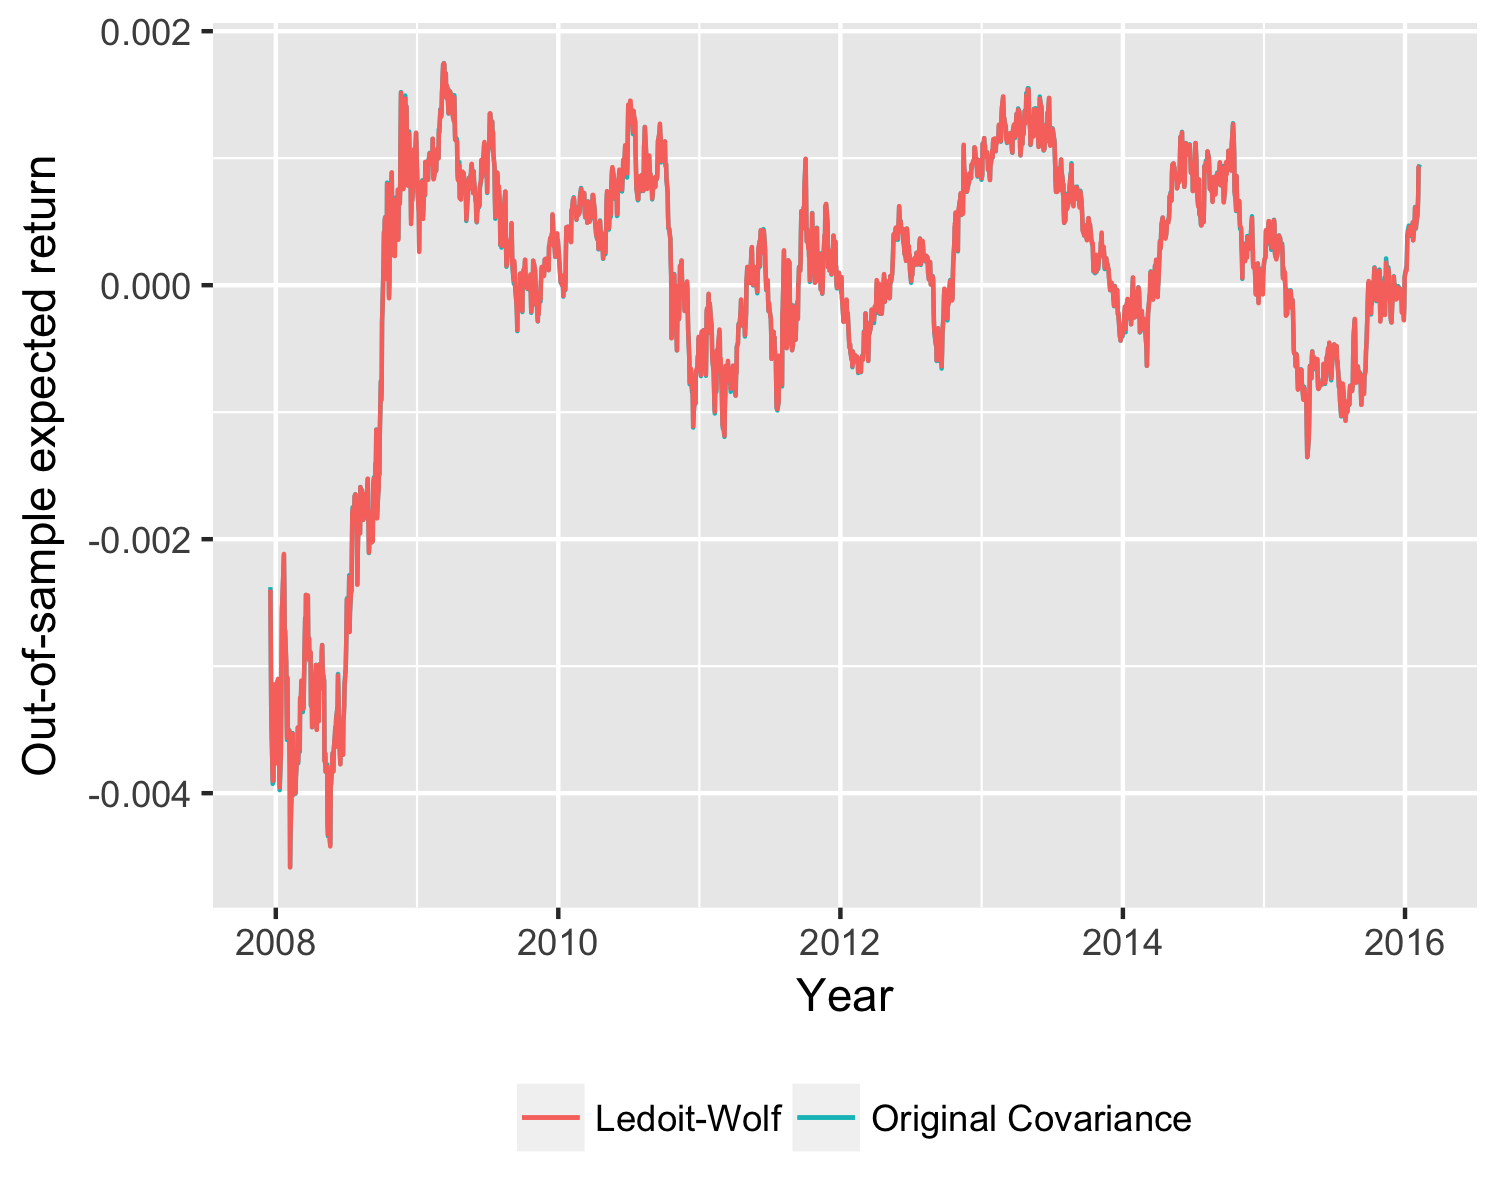
\includegraphics[width=\textwidth]{fig_mean_variance_ous_r.png}
    \caption{Out of sample expected returns (mean-variance portfolio).\label{fig:fig_mean_variance_ous_r}}
  \end{minipage}
  \hfill
  \begin{minipage}[t]{0.45\textwidth}
    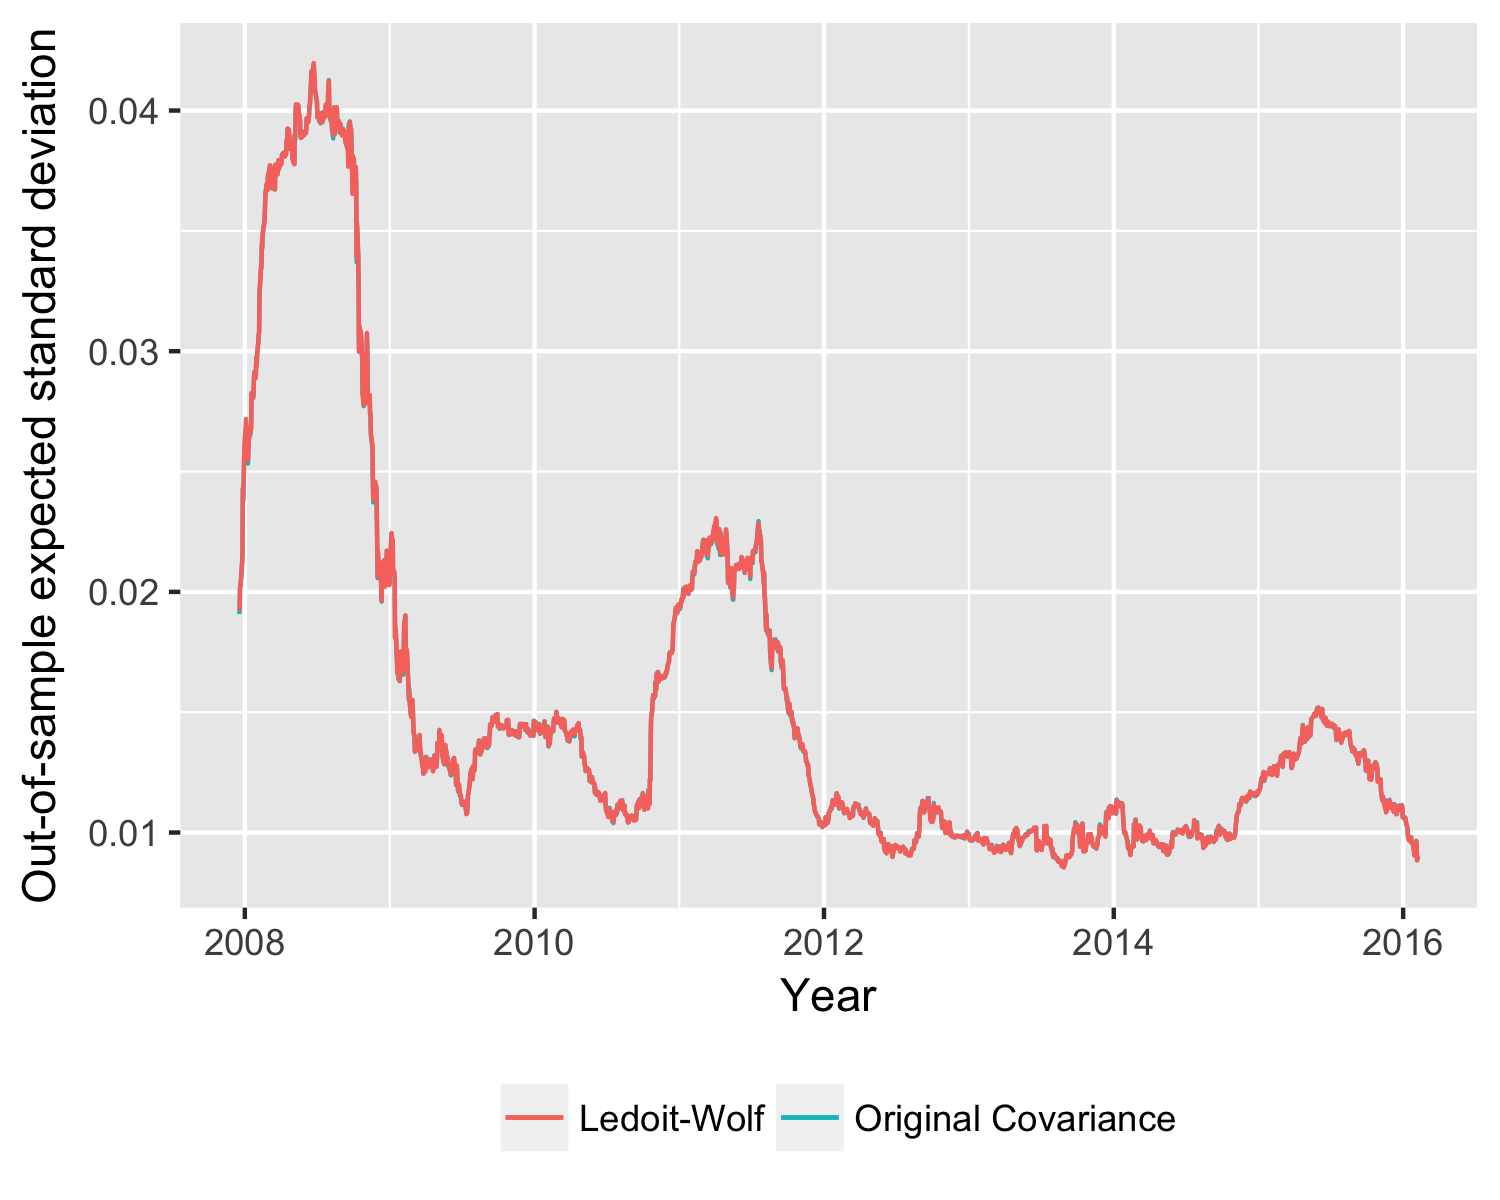
\includegraphics[width=\textwidth]{fig_mean_variance_ous_std.png}
    \caption{Out of sample expected standard deviations (mean-variance portfolio).\label{fig:fig_mean_variance_ous_std}}
  \end{minipage}
\end{figure}

\begin{figure}
  \centering
    \centering{%
      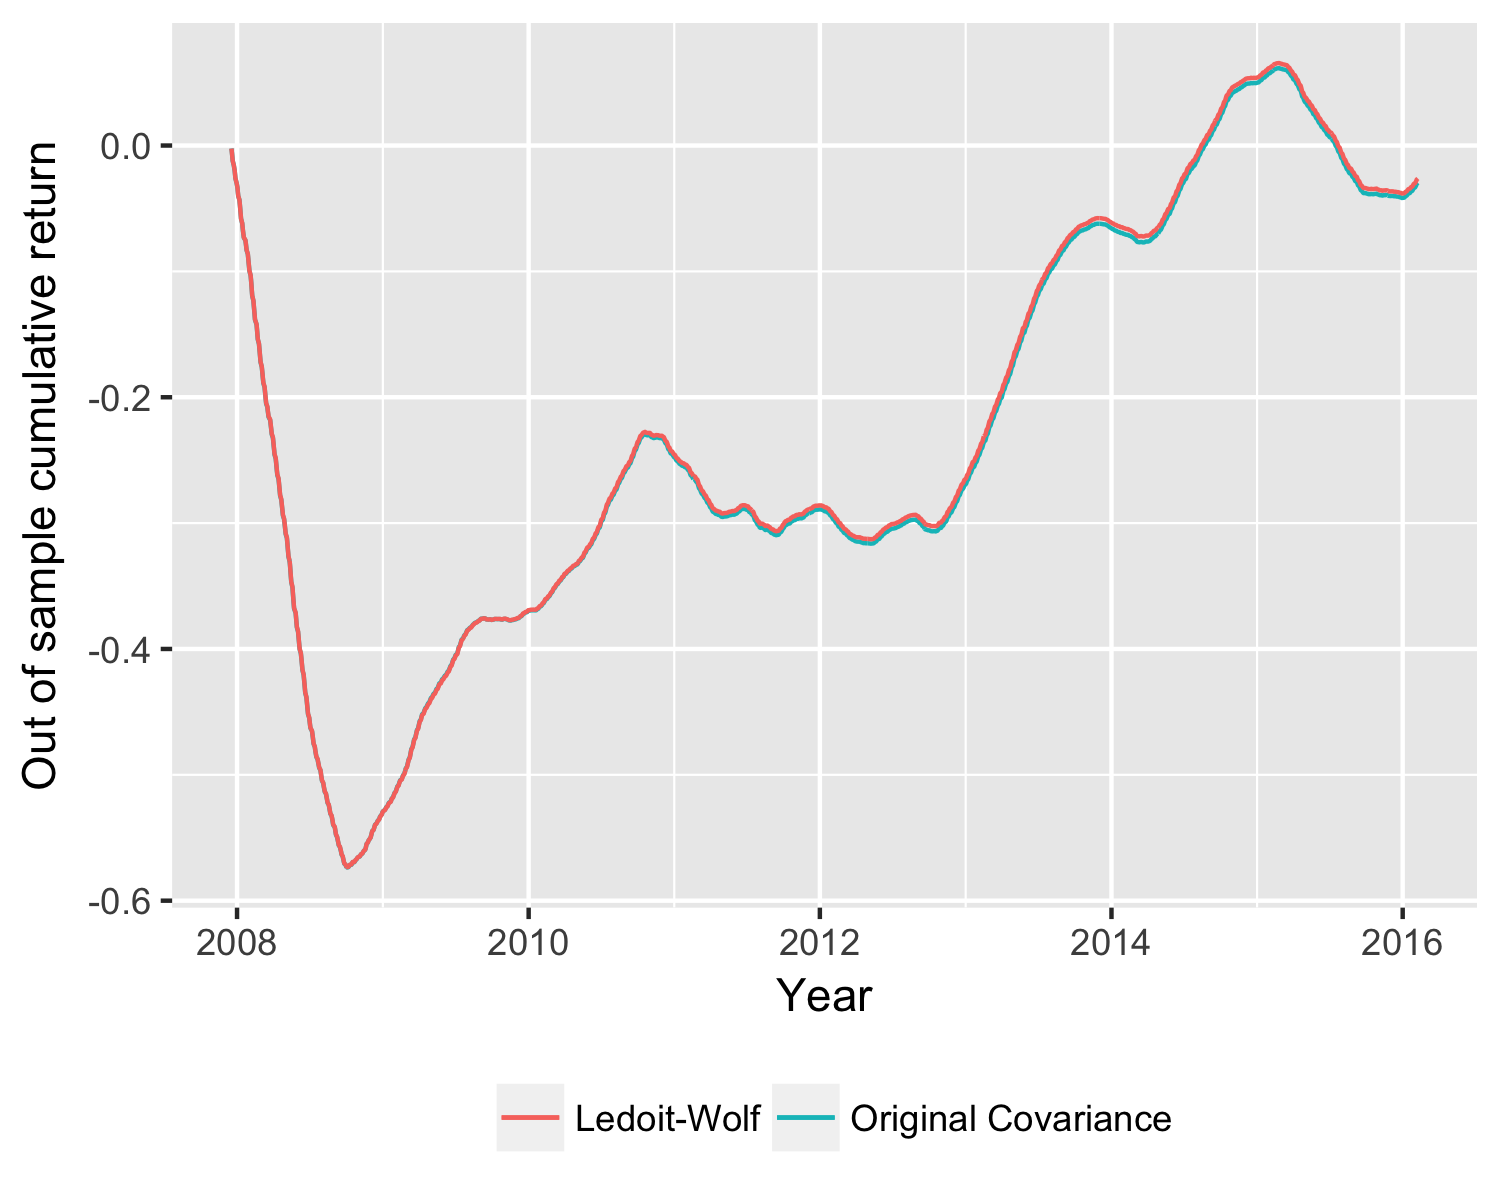
\includegraphics[width=0.45\textwidth]{fig_mean_variance_cum.png}}
  \caption{Out of sample cumulative expected return (mean-variance portfolio).\label{fig:fig_mean_variance_cum}}
\end{figure}

\subsection{Comparison}
In all cases when we use the transformed covariance matrix through shrinkage ~\cite{LW}, that gives better results compared to the results when we use the original covariance matrix. The minimum-variance portfolio which only goal was to minimize the variance outperforms the mean-variance portfolio. In the case of mean-variance portfolio, the results are almost equal for both covariance matrices. Also the fact that it tries to reach a previously specified expected return has a negative impact on the results because it does not diversify enough and as a result it performs poorly in the evaluation sample.

\section{Machine Learning for forecasting financial time series}

In this section we present two popular machine learning techniques, namely SVM (support vector machines) ~\cite{SVM} and NN (neural networks) ~\cite{NN}. We use them both of them in order to predict the annual returns of S\&P500 and APPLE and compare them to conclude which method gives more accurate predictions.

\subsection{SVM}
SVMs are among the best "off-the-shelf" supervised learning algorithm that can be used for classification and regression analysis. Since we want to predict the returns of a time series we use SVMs for regression analysis. To use this method we need to create features. One good way to do this is by lagging the time series of returns. So our 4 features are lags 1, 2, 3, 5 of the time series. SVMs are characterized by parameters that we need to tune. The most 2 important parameters are the kernel function and the cost. By testing and using all available kernel functions we ended up to the linear kernel. The optimal value for C (cost) is equal to one. One important thing is that SVM gives very good predictions when we use as input the rolling \textbf{annual returns} and not the daily or the weekly returns. So in our analysis we use the annual returns as input in order to create the features and then to predict annual returns. We use root mean square error (RMSE) to evaluate our model. The results are presented in Table \ref{table:tbl2}. RMSE for both S\&P500 and APPLE are low, that is our model predicts the annual returns accurately. In figures \ref{fig:figSVMSP500}, \ref{fig:figSVMAPPLE} we can see an almost straight line between the values of actual returns and the corresponding predicted values. The low values of RMSE for both S\&P500 and APPLE and the two figures are a good sign that our model can predict the future annual returns with high accuracy.

\begin{figure}[!tbp]
  \centering
  \begin{minipage}[t]{0.45\textwidth}
    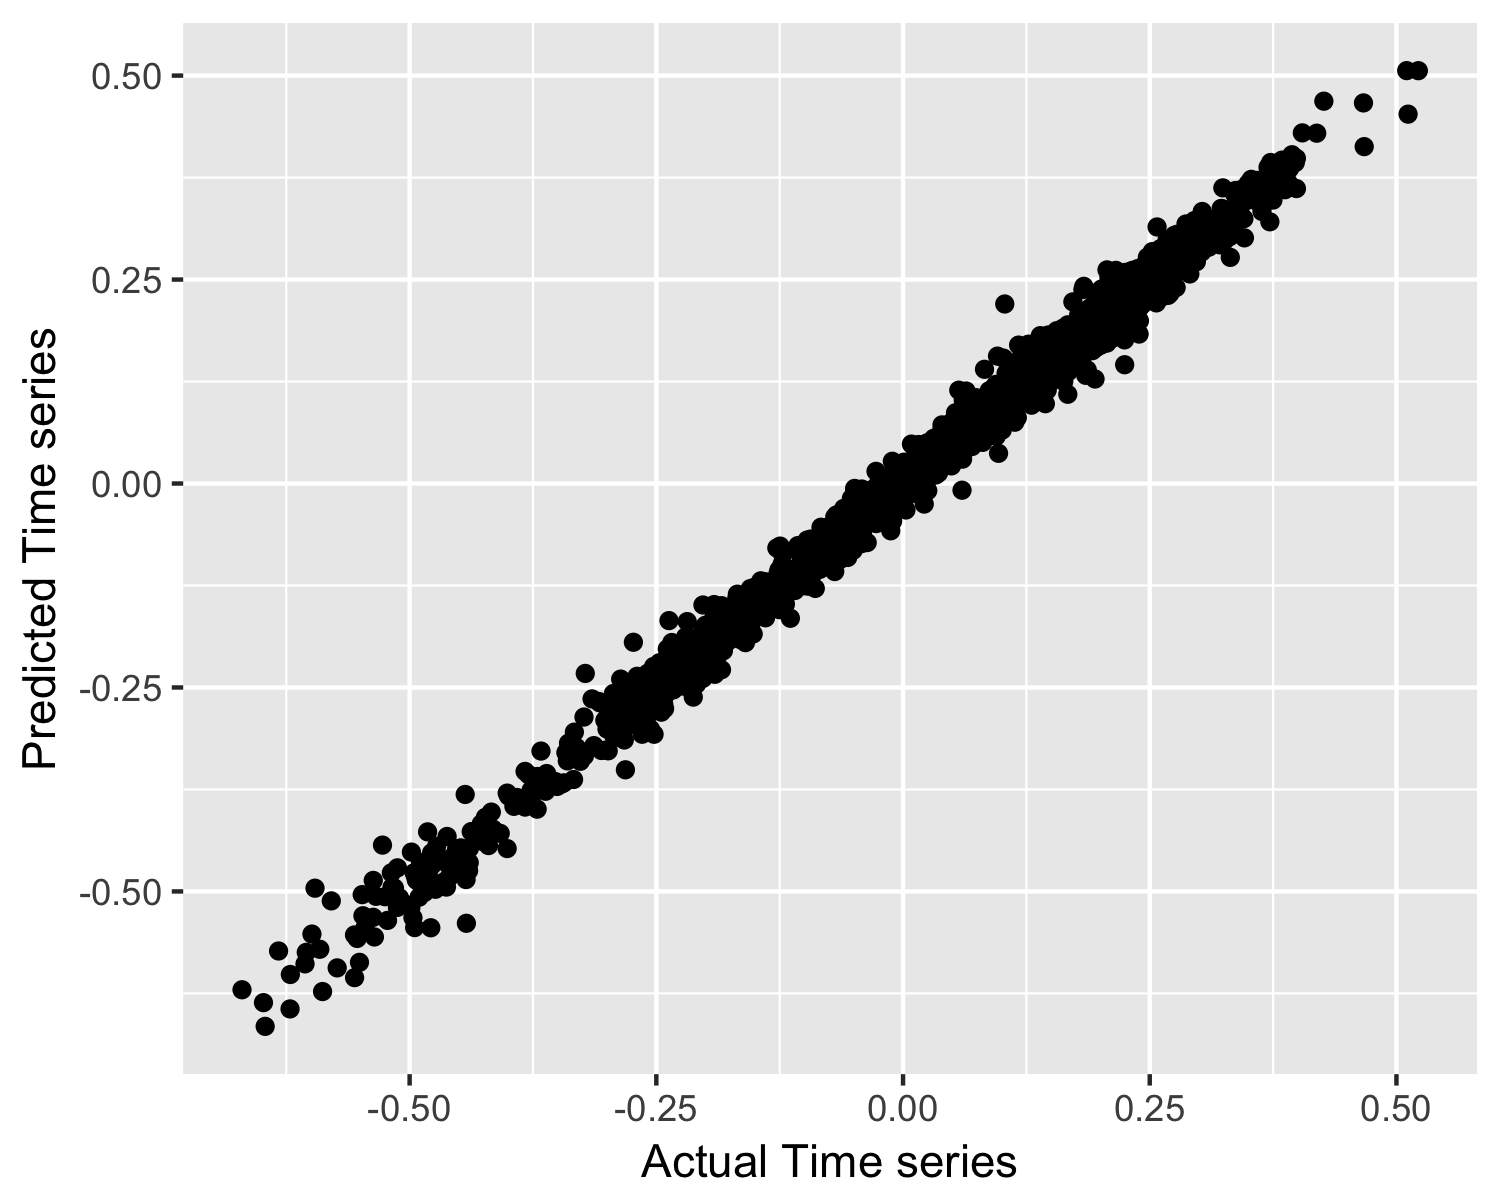
\includegraphics[width=\textwidth]{figSVMSP500.png}
    \caption{Predicted value with the corresponding real value of returns for S\&P500.\label{fig:figSVMSP500}}
  \end{minipage}
  \hfill
  \begin{minipage}[t]{0.45\textwidth}
    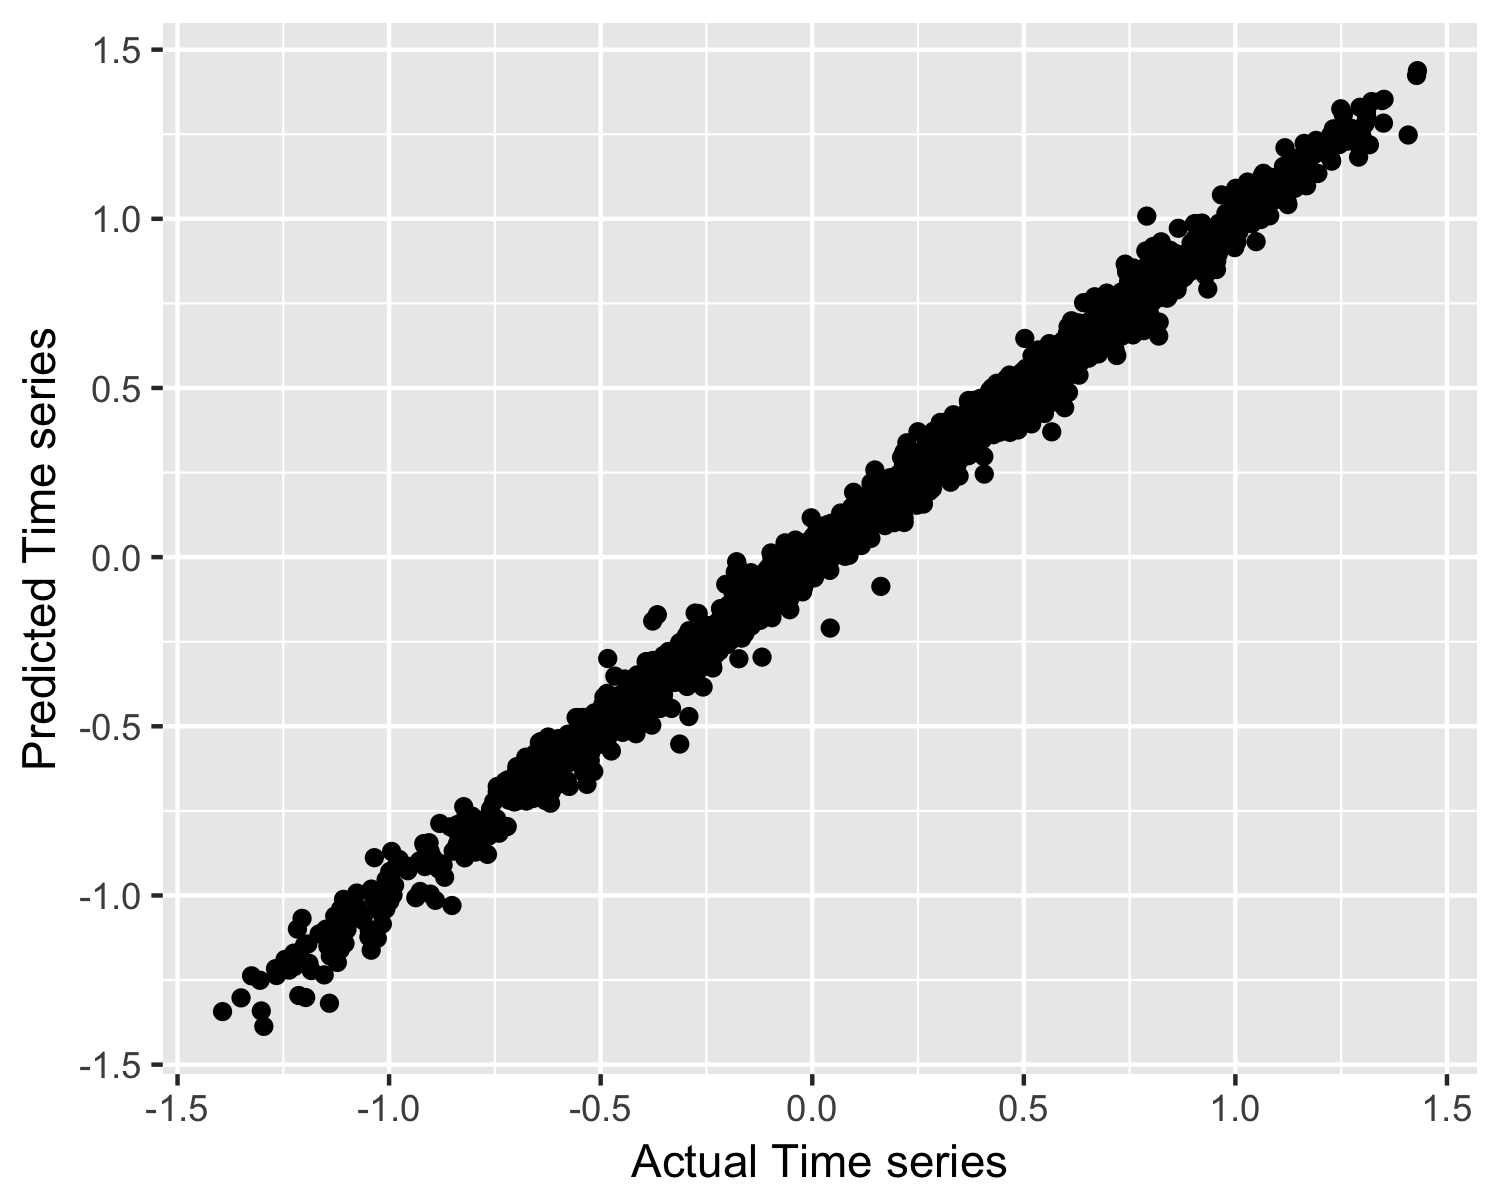
\includegraphics[width=\textwidth]{figSVMAPPLE.png}
    \caption{Predicted value with the corresponding real value of returns for APPLE.\label{fig:figSVMAPPLE}}
  \end{minipage}
\end{figure}

\subsection{NN}

Neural networks are organized in layers. Layers are made up of a number of interconnected nodes which contain an activation function. Patterns are presented to the network via the input layer, which communicates to one or more hidden layers where the actual processing is done via a system of weighted connections. The hidden layers then link to an output layer where the output is the answer. As before, we use the rolling \textbf{annual returns} because they give better predictions. We create from the annual returns, 4 features (lags 1, 2, 3, 5), so our neural network needs to have 4 neurons in the input layer. NN are characterized by parameters that we need to tune. The most 2 important parameters are the number of hidden layers and the weights decay. By testing we ended up to use 1 hidden layer of one neuron. Regarding weights decays, it is equal to 0.001 for S\&P500 and 0 for APPLE. We use root mean square error (RMSE) to evaluate our model. The results are presented in Table \ref{table:tbl2}. RMSE for both S\&P500 and APPLE are low, that is our model predicts the annual returns accurately. In figures \ref{fig:figNNSP500}, \ref{fig:figNNAPPLE} we can see an almost straight line between the values of actual returns and the corresponding predicted values. The low values of RMSE for both S\&P500 and APPLE and the two figures are a good sign that our model can predict the future annual returns with high accuracy.


\begin{figure}[!tbp]
  \centering
  \begin{minipage}[t]{0.45\textwidth}
    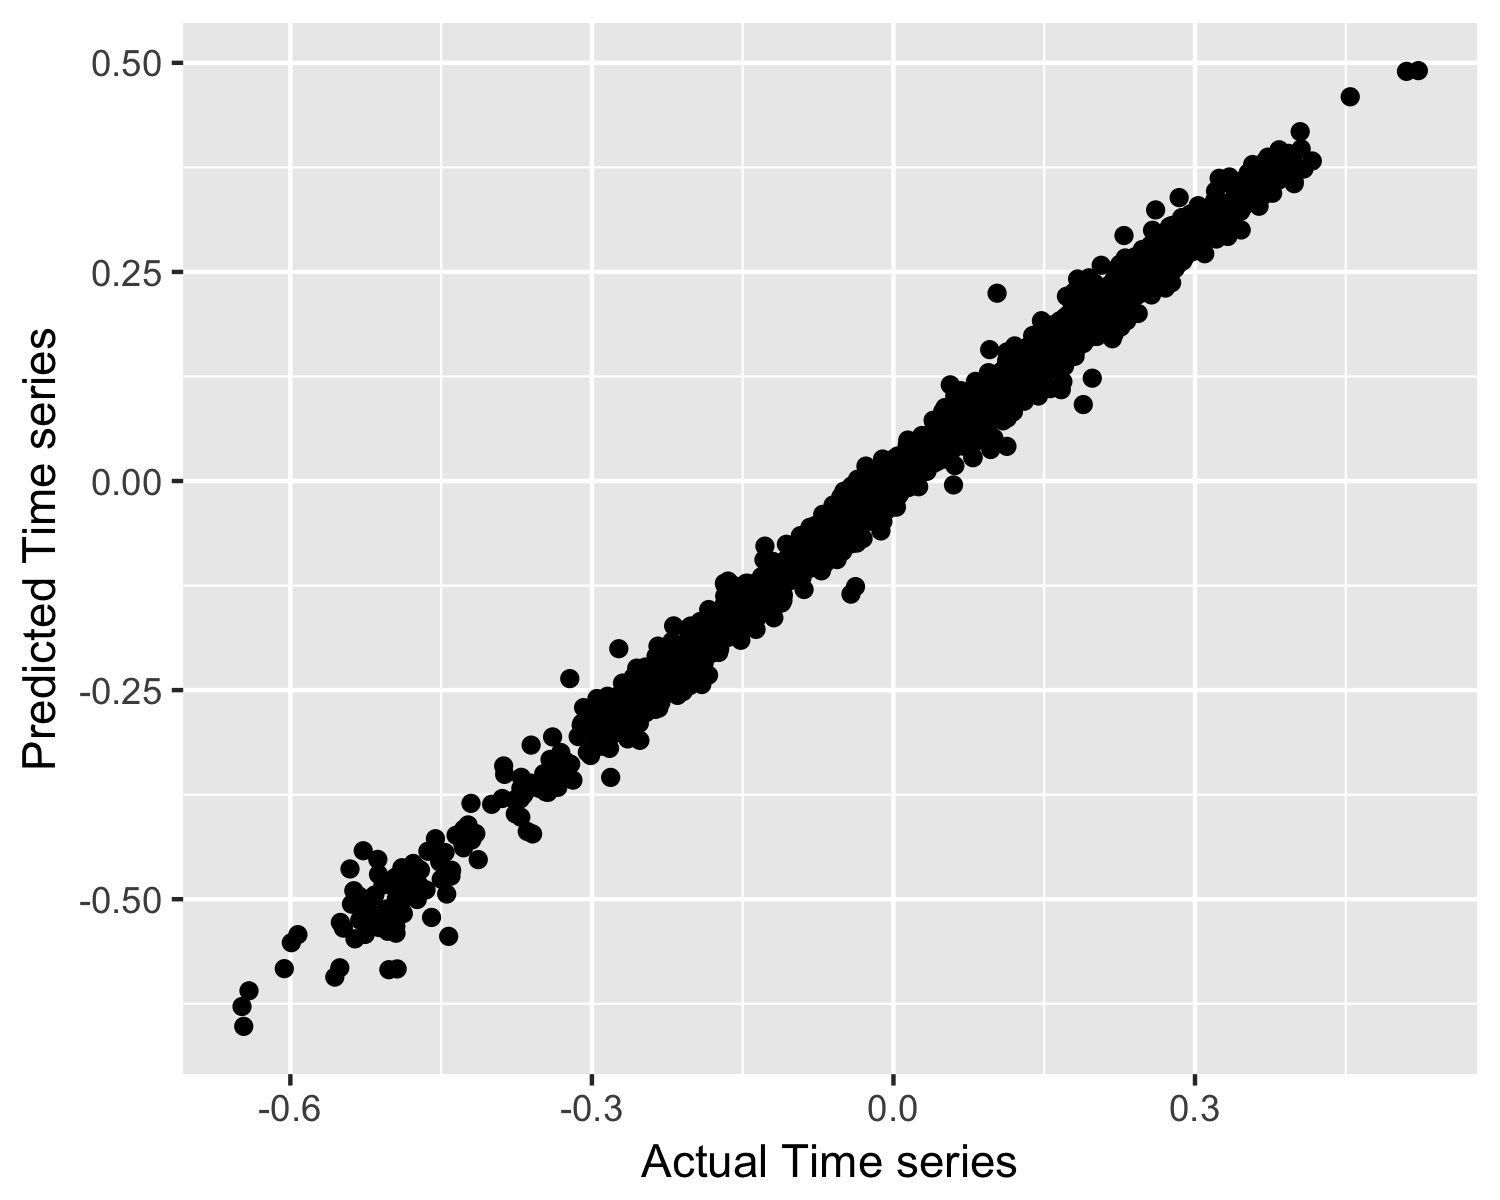
\includegraphics[width=\textwidth]{figNNSP500.png}
    \caption{Predicted value with the corresponding real value of returns for S\&P500.\label{fig:figNNSP500}}
  \end{minipage}
  \hfill
  \begin{minipage}[t]{0.45\textwidth}
    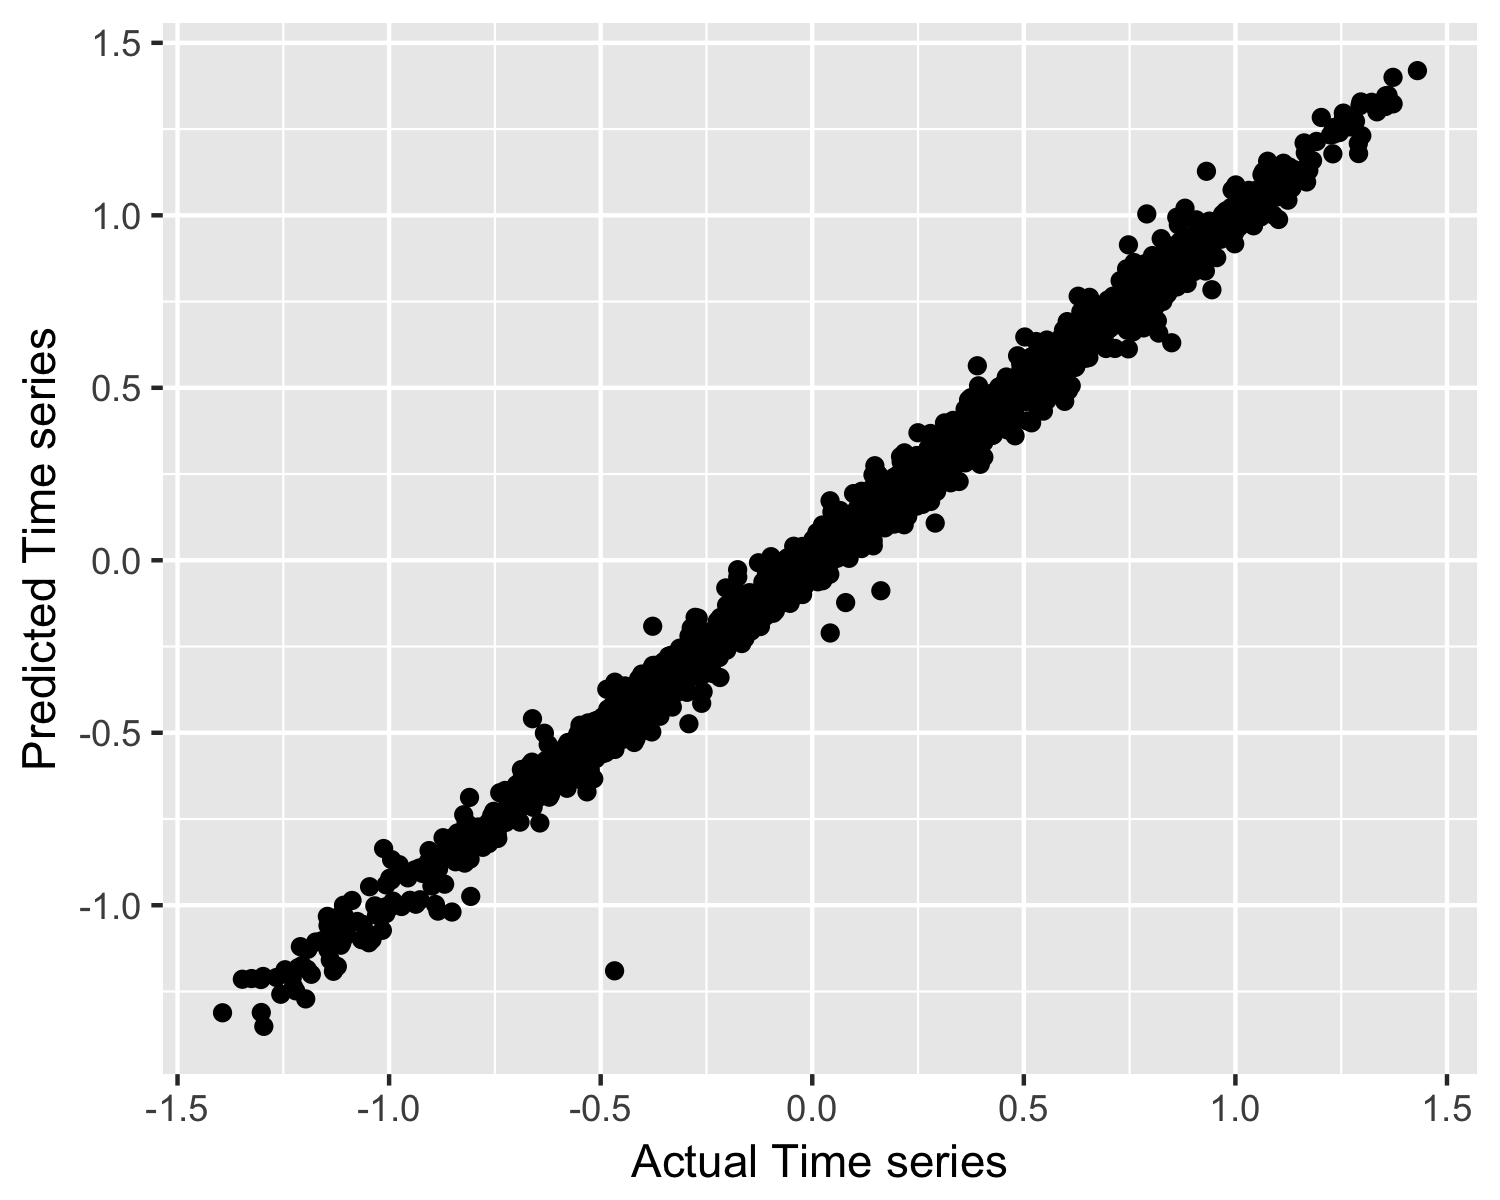
\includegraphics[width=\textwidth]{figNNAPPLE.png}
    \caption{Predicted value with the corresponding real value of returns for APPLE.\label{fig:figNNAPPLE}}
  \end{minipage}
\end{figure}


\subsection{Comparison}

From Table \ref{table:tbl2} it is obvious that both support vector machines and neural networks provide very good results. The fact that RMSE is a little smaller in SVM does not provide a certainty that SVM gives more accurate results. It is possible that this little difference in values is caused by luck. 

\begin{table}[]
\centering
\caption{Comparing the accuracy of the 2 models}
\label{table:tbl2}
\begin{tabular}{ccc}
\hline
\textbf{\begin{tabular}[c]{@{}c@{}}Machine \\ Learning\\ Technique\end{tabular}} & \textbf{\begin{tabular}[c]{@{}c@{}}RMSE\\ S\&P500\end{tabular}} & \textbf{\begin{tabular}[c]{@{}c@{}}RMSE\\ APPLE\end{tabular}} \\ \hline
\begin{tabular}[c]{@{}c@{}}SVM, linear kernel,\\ C = 1\end{tabular}              &0.01635442                                                                 &0.0401503                                                               \\ \hline
NN, 1 hidden layer, \\ decay = 0.001, \\ (decay = 0 for APPLE)                                                              &0.01640119                                                                 &0.04210067                                                               \\ \hline
\end{tabular}
\end{table}

\section{Conclusions}
Our analysis leads us to choose the minimum-variance portfolio and SVM or NN as the best ways to optimize our portfolio.

\begin{thebibliography}{99}

\bibitem{Rama}
Cont, R. (2001). Empirical properties of asset returns: stylized facts and statistical issues. Quantitative Finance, 1, 223-236.

\bibitem{Campbell}
Campbell, J., Lo, A., MacKinlay, A. (1997). The Econometrics of Financial Markets. Princeton: Princeton University Press.

\bibitem{Mandelbrot}
Mandelbrot, B. (1963). The variation of certain speculative prices. Journal of Business, 35, 394.

\bibitem{Markowitz}
\href{https://en.wikipedia.org/wiki/Modern_portfolio_theory}{Modern portfolio theory by Harry Markowitz}

\bibitem{Asset}
\href{https://en.wikipedia.org/wiki/Asset_allocation}{Asset Allocation}

\bibitem{Min-variance}
Roger G Clarke, Harindra de Silva, and Steven Thorley. Minimum-Variance Portfolios in the U.S. Equity Market. The Journal of Portfolio Management,
Fall 2006, Vol. 33, No. 1: pp. 10-24

\bibitem{WGCNA}
Langfelder P, Horvath S (2008) WGCNA: an R package for weighted correlation network analysis. BMC Bioinformatics 2008, 9:559

\bibitem{LW}
Olivier Ledoit, Michael Wolf. Honey, I Shrunk the Sample Covariance Matrix. The Journal of Portfolio Management, 2004, Vol 30, No. 4: pp. 110-119

\bibitem{SVM}
\href{https://en.wikipedia.org/wiki/Support_vector_machine}{Support Vector Machines}

\bibitem{NN}
\href{https://en.wikipedia.org/wiki/Artificial_neural_network}{Neural Networks}


\end{thebibliography}


\end{document}
